\documentclass[]{book}
\usepackage{lmodern}
\usepackage{amssymb,amsmath}
\usepackage{ifxetex,ifluatex}
\usepackage{fixltx2e} % provides \textsubscript
\ifnum 0\ifxetex 1\fi\ifluatex 1\fi=0 % if pdftex
  \usepackage[T1]{fontenc}
  \usepackage[utf8]{inputenc}
\else % if luatex or xelatex
  \ifxetex
    \usepackage{mathspec}
  \else
    \usepackage{fontspec}
  \fi
  \defaultfontfeatures{Ligatures=TeX,Scale=MatchLowercase}
\fi
% use upquote if available, for straight quotes in verbatim environments
\IfFileExists{upquote.sty}{\usepackage{upquote}}{}
% use microtype if available
\IfFileExists{microtype.sty}{%
\usepackage{microtype}
\UseMicrotypeSet[protrusion]{basicmath} % disable protrusion for tt fonts
}{}
\usepackage[margin=1in]{geometry}
\usepackage{hyperref}
\hypersetup{unicode=true,
            pdftitle={CHEM 191 Workbook: Building a Teensy Air Quality Monitor},
            pdfauthor={Al Fischer},
            pdfborder={0 0 0},
            breaklinks=true}
\urlstyle{same}  % don't use monospace font for urls
\usepackage{natbib}
\bibliographystyle{apalike}
\usepackage{color}
\usepackage{fancyvrb}
\newcommand{\VerbBar}{|}
\newcommand{\VERB}{\Verb[commandchars=\\\{\}]}
\DefineVerbatimEnvironment{Highlighting}{Verbatim}{commandchars=\\\{\}}
% Add ',fontsize=\small' for more characters per line
\usepackage{framed}
\definecolor{shadecolor}{RGB}{248,248,248}
\newenvironment{Shaded}{\begin{snugshade}}{\end{snugshade}}
\newcommand{\AlertTok}[1]{\textcolor[rgb]{0.94,0.16,0.16}{#1}}
\newcommand{\AnnotationTok}[1]{\textcolor[rgb]{0.56,0.35,0.01}{\textbf{\textit{#1}}}}
\newcommand{\AttributeTok}[1]{\textcolor[rgb]{0.77,0.63,0.00}{#1}}
\newcommand{\BaseNTok}[1]{\textcolor[rgb]{0.00,0.00,0.81}{#1}}
\newcommand{\BuiltInTok}[1]{#1}
\newcommand{\CharTok}[1]{\textcolor[rgb]{0.31,0.60,0.02}{#1}}
\newcommand{\CommentTok}[1]{\textcolor[rgb]{0.56,0.35,0.01}{\textit{#1}}}
\newcommand{\CommentVarTok}[1]{\textcolor[rgb]{0.56,0.35,0.01}{\textbf{\textit{#1}}}}
\newcommand{\ConstantTok}[1]{\textcolor[rgb]{0.00,0.00,0.00}{#1}}
\newcommand{\ControlFlowTok}[1]{\textcolor[rgb]{0.13,0.29,0.53}{\textbf{#1}}}
\newcommand{\DataTypeTok}[1]{\textcolor[rgb]{0.13,0.29,0.53}{#1}}
\newcommand{\DecValTok}[1]{\textcolor[rgb]{0.00,0.00,0.81}{#1}}
\newcommand{\DocumentationTok}[1]{\textcolor[rgb]{0.56,0.35,0.01}{\textbf{\textit{#1}}}}
\newcommand{\ErrorTok}[1]{\textcolor[rgb]{0.64,0.00,0.00}{\textbf{#1}}}
\newcommand{\ExtensionTok}[1]{#1}
\newcommand{\FloatTok}[1]{\textcolor[rgb]{0.00,0.00,0.81}{#1}}
\newcommand{\FunctionTok}[1]{\textcolor[rgb]{0.00,0.00,0.00}{#1}}
\newcommand{\ImportTok}[1]{#1}
\newcommand{\InformationTok}[1]{\textcolor[rgb]{0.56,0.35,0.01}{\textbf{\textit{#1}}}}
\newcommand{\KeywordTok}[1]{\textcolor[rgb]{0.13,0.29,0.53}{\textbf{#1}}}
\newcommand{\NormalTok}[1]{#1}
\newcommand{\OperatorTok}[1]{\textcolor[rgb]{0.81,0.36,0.00}{\textbf{#1}}}
\newcommand{\OtherTok}[1]{\textcolor[rgb]{0.56,0.35,0.01}{#1}}
\newcommand{\PreprocessorTok}[1]{\textcolor[rgb]{0.56,0.35,0.01}{\textit{#1}}}
\newcommand{\RegionMarkerTok}[1]{#1}
\newcommand{\SpecialCharTok}[1]{\textcolor[rgb]{0.00,0.00,0.00}{#1}}
\newcommand{\SpecialStringTok}[1]{\textcolor[rgb]{0.31,0.60,0.02}{#1}}
\newcommand{\StringTok}[1]{\textcolor[rgb]{0.31,0.60,0.02}{#1}}
\newcommand{\VariableTok}[1]{\textcolor[rgb]{0.00,0.00,0.00}{#1}}
\newcommand{\VerbatimStringTok}[1]{\textcolor[rgb]{0.31,0.60,0.02}{#1}}
\newcommand{\WarningTok}[1]{\textcolor[rgb]{0.56,0.35,0.01}{\textbf{\textit{#1}}}}
\usepackage{longtable,booktabs}
\usepackage{graphicx,grffile}
\makeatletter
\def\maxwidth{\ifdim\Gin@nat@width>\linewidth\linewidth\else\Gin@nat@width\fi}
\def\maxheight{\ifdim\Gin@nat@height>\textheight\textheight\else\Gin@nat@height\fi}
\makeatother
% Scale images if necessary, so that they will not overflow the page
% margins by default, and it is still possible to overwrite the defaults
% using explicit options in \includegraphics[width, height, ...]{}
\setkeys{Gin}{width=\maxwidth,height=\maxheight,keepaspectratio}
\IfFileExists{parskip.sty}{%
\usepackage{parskip}
}{% else
\setlength{\parindent}{0pt}
\setlength{\parskip}{6pt plus 2pt minus 1pt}
}
\setlength{\emergencystretch}{3em}  % prevent overfull lines
\providecommand{\tightlist}{%
  \setlength{\itemsep}{0pt}\setlength{\parskip}{0pt}}
\setcounter{secnumdepth}{5}
% Redefines (sub)paragraphs to behave more like sections
\ifx\paragraph\undefined\else
\let\oldparagraph\paragraph
\renewcommand{\paragraph}[1]{\oldparagraph{#1}\mbox{}}
\fi
\ifx\subparagraph\undefined\else
\let\oldsubparagraph\subparagraph
\renewcommand{\subparagraph}[1]{\oldsubparagraph{#1}\mbox{}}
\fi

%%% Use protect on footnotes to avoid problems with footnotes in titles
\let\rmarkdownfootnote\footnote%
\def\footnote{\protect\rmarkdownfootnote}

%%% Change title format to be more compact
\usepackage{titling}

% Create subtitle command for use in maketitle
\providecommand{\subtitle}[1]{
  \posttitle{
    \begin{center}\large#1\end{center}
    }
}

\setlength{\droptitle}{-2em}

  \title{CHEM 191 Workbook: Building a Teensy Air Quality Monitor}
    \pretitle{\vspace{\droptitle}\centering\huge}
  \posttitle{\par}
    \author{Al Fischer}
    \preauthor{\centering\large\emph}
  \postauthor{\par}
      \predate{\centering\large\emph}
  \postdate{\par}
    \date{Western Carolina University}


\begin{document}
\maketitle

{
\setcounter{tocdepth}{1}
\tableofcontents
}
\hypertarget{section}{%
\chapter*{}\label{section}}
\addcontentsline{toc}{chapter}{}

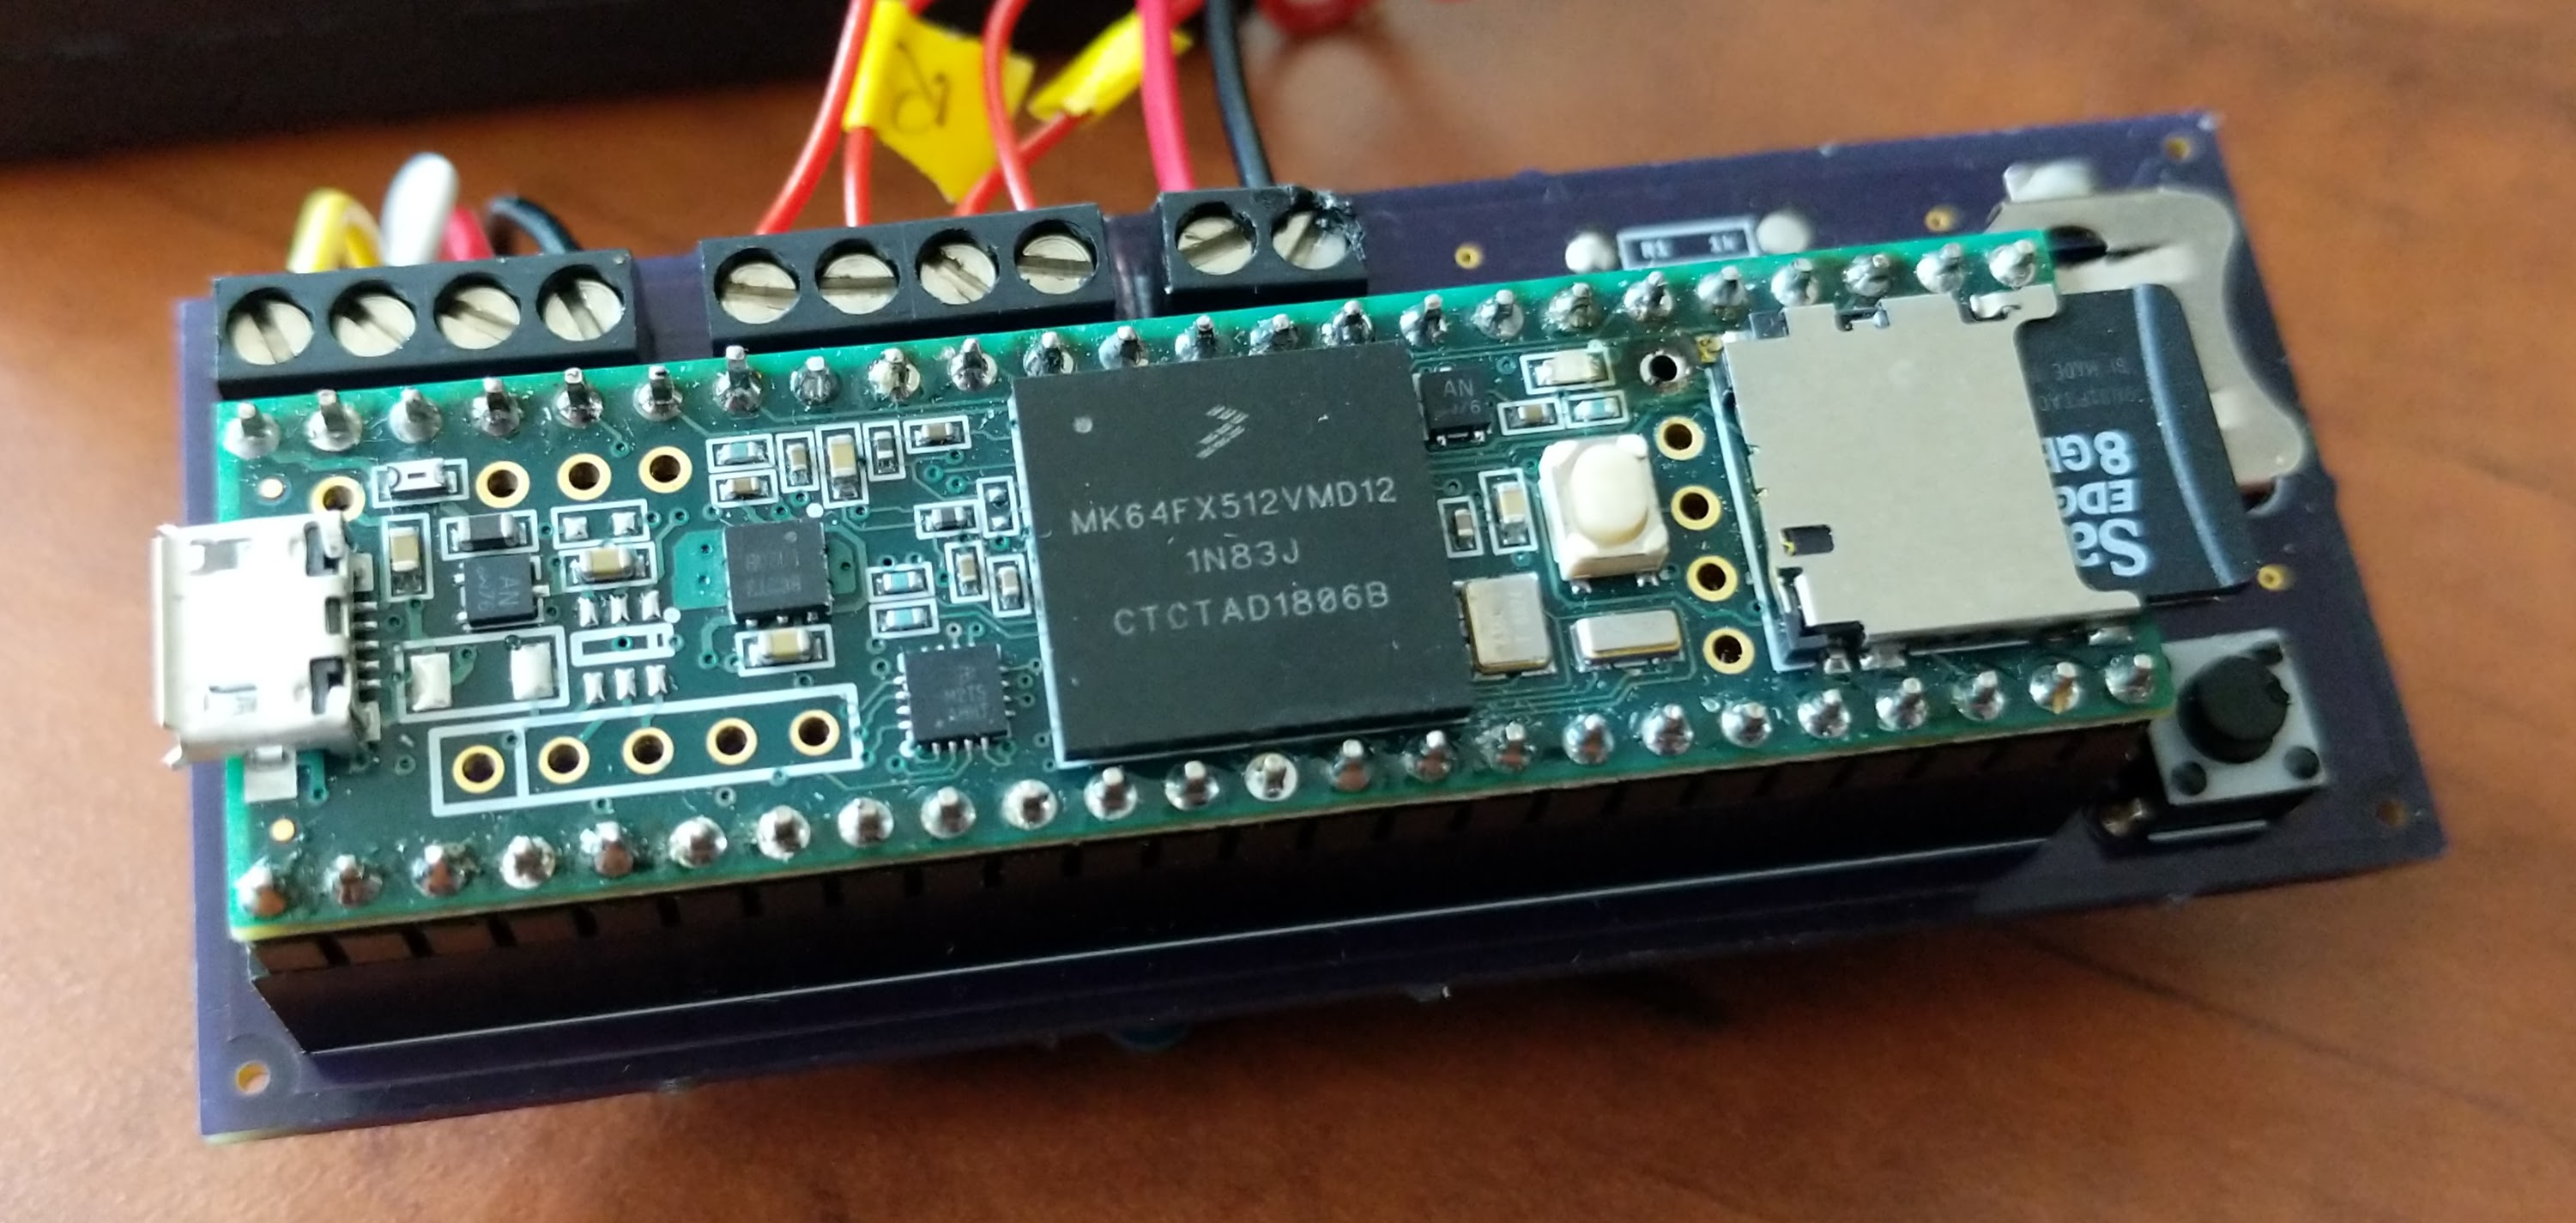
\includegraphics{images/teensy_aqm.jpg}

\emph{Copyright 2019 Al Fischer. This work is released under the \href{https://creativecommons.org/licenses/by-sa/4.0/}{CC-BY-NC-SA 4.0 license}.}

\hypertarget{preface}{%
\chapter*{Preface}\label{preface}}
\addcontentsline{toc}{chapter}{Preface}

\hypertarget{what-is-arduino}{%
\section*{What is Arduino?}\label{what-is-arduino}}
\addcontentsline{toc}{section}{What is Arduino?}

Over the course of the semester, we will build air quality monitors using the Teensy microcontroller platform. This platform is an offshoot of the popular Arduino microcontrollers, and they are very similar. This workbook will introduce you to the basics of Arduino and Teensy, and walk you through assembling and programming your air quality sensor.

\textbf{Arduino} is an \href{http://www.wikipedia.com/wiki/Open-source}{open-source} platform for developing interactive electronic devices. Arduinos of various flavors are used for all variety of things, from controlling motors and lights to reading data from sensors. Exercise 1 will provide a more thorough overview of Arduino.

\hypertarget{ok-but-what-is-teensy}{%
\section*{OK, but what is Teensy?}\label{ok-but-what-is-teensy}}
\addcontentsline{toc}{section}{OK, but what is Teensy?}

Teensy is an offshoot of Arduino. It is capapble of most everything an Arduino can do and often much more. You might think of it as the supercar version of an Arduino. Aside from being more capable, it's also smaller -- a fact that gives rise to it's name (Teensy). In this class, the names Teensy and Arduino will be used interchangeably. Exercise 1 will provide a more thorough overview of Teensy.

\hypertarget{using-this-book}{%
\section*{Using this Book}\label{using-this-book}}
\addcontentsline{toc}{section}{Using this Book}

Some common typographical (formatting) conventions will be used throughout this book.

\hypertarget{code}{%
\subsection*{Code}\label{code}}
\addcontentsline{toc}{subsection}{Code}

The exercises will make extensive use of computer code, which will always be represented with \texttt{monospace} font with a grey background. It may be \texttt{inline} or

\begin{verbatim}
offset.
\end{verbatim}

When you see code, you should take time to thoroughly digest it. Sometimes the code may work as-is; other times you may have to add to the code to make it work. And other times the code may be \texttt{pseudocode}, which is example code that looks like it would work but will not actually compile. The code will often be color-coded to highlight various features of the programming language.

\hypertarget{notes-and-warnings}{%
\subsection*{Notes and Warnings}\label{notes-and-warnings}}
\addcontentsline{toc}{subsection}{Notes and Warnings}

This book will also make use of notes and warnings. Examples are below.

\begin{quote}
\emph{A note is written in a quote box with italic font and represents background information or a bit of knowledge to think about.}
\end{quote}

\begin{quote}
A NOTE ALL CAPITAL LETTERS REPRESENTS A SAFETY WARNING. YOU \textbf{MUST} PAY ATTENTION TO THESE WARNING OR YOU MAY BREAK EQUIPMENT AND/OR HARM YOURSELF OR YOUR CLASSMATES.
\end{quote}

\hypertarget{is-this-work-dangerous}{%
\section*{Is this work dangerous?}\label{is-this-work-dangerous}}
\addcontentsline{toc}{section}{Is this work dangerous?}

Although electricity can be very dangerous and even lethal, the work we'll do in this class shouldn't pose any particular danger if done carefully. There are two important factors to consider when deciding how dangerous an electrical device is: (1) the voltage and (2) the current. Generally speaking, it takes both to be dangerous. Most of the voltage in these exercises will be either 3.3V or 5V, with currents on the order of 100 mA. These are relatively low voltages and low currents, are safe to work with, and do not pose a shock hazard. That said, connecting things incorrectly can still break components, cause them to get very hot (they might burn you), or even go up in smoke -- be careful and double check yourself/your lab partner when connecting things!

\hypertarget{additional-resources}{%
\section*{Additional Resources}\label{additional-resources}}
\addcontentsline{toc}{section}{Additional Resources}

There are myriad books, blog posts, and websites about Arduino, but few specifically deal with the Teensy version. This workbook and the \href{http://www.pjrc.com}{Teensy website} are your best resources regarding Teensy-specific items. The code used to program the Teensy (and Arduinos) is a version of \texttt{C}; knowing that will be useful when trying to find help online. The \href{https://www.arduino.cc/reference/en/}{Arduino language reference} provides a list of available functionalities and syntax.

If you want more general information on programming Arduinos, the Arduino IDE, or electronics, you may check some of the following:

\begin{itemize}
\tightlist
\item
  Monk, Simon. \href{https://www.amazon.com/Programming-Arduino-Getting-Started-Sketches/dp/0071784225}{\textbf{\emph{Programming Arduino: Getting Started with Sketches}}}.\\
\item
  Scherz, Paul and Simon Monk. \href{https://www.amazon.com/Practical-Electronics-Inventors-Fourth-Scherz/dp/1259587541/ref=pd_lpo_sbs_14_t_0?_encoding=UTF8\&psc=1\&refRID=9JN842FPFMNAA9RQV8X3}{\textbf{\emph{Practical Electronics for Inventors}}}.\\
\item
  The Arduino \href{https://forum.arduino.cc/}{forum}.\\
\item
  Boxall, John. \href{https://www.amazon.com/Arduino-Workshop-Hands-Introduction-Projects/dp/1593274483}{\textbf{\emph{Arduino Workshop}}}.
\end{itemize}

\hypertarget{getting-started-with-arduino}{%
\chapter{Getting Started with Arduino}\label{getting-started-with-arduino}}

\textbf{Objective:} Install Arduino and Teensyduino\\
\textbf{To turn in:} Nothing! Make sure your software is installed and working so you're ready for the next class period.

\hypertarget{introduction}{%
\section*{Introduction}\label{introduction}}
\addcontentsline{toc}{section}{Introduction}

\textbf{Arduino} is an \href{http://www.wikipedia.com/wiki/Open-source}{open-source} platform for developing interactive electronic devices. More specifically, Arduinos are \href{https://en.wikipedia.org/wiki/Microcontroller}{\emph{microcontrollers}}, which are essentially small computers that can be programmed to perform a specific task over and over again. Microcontrollers are ubiquitous in the modern world and are embedded in scientific equipment, cars, cell phones, and nearly every other electronic device. Arduino provides a simple, standardized interface for microcontrollers, which has led it to become a very popular tool for hobby projects, citizen science tools, and even art installations. Arduino began in 2005 as a student project at the Interaction Design Institute Ivrea in Ivrea, Italy.

\begin{figure}
\centering
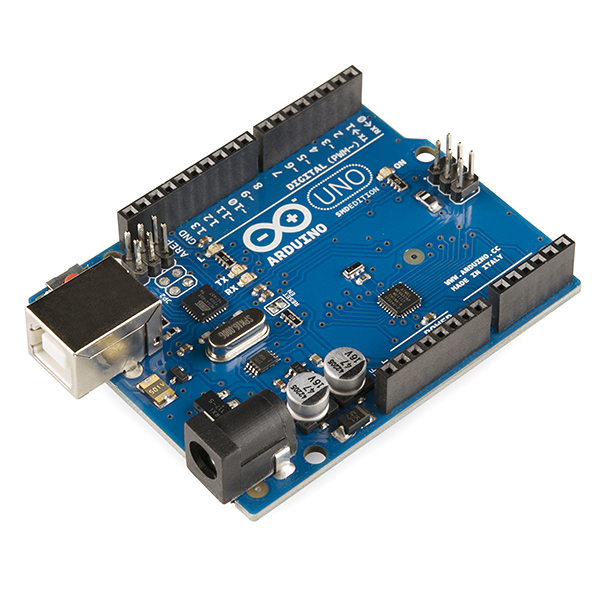
\includegraphics{images/Arduino_Uno_-_R3.jpg}
\caption{\emph{An Arduino Uno. This class will use a variant of the Arduino, called the Teensy, as described below. (image credit: \href{https://commons.wikimedia.org/wiki/File:Arduino_Uno_-_R3.jpg}{Spark Fun, CC BY 2.0})}}
\end{figure}

Using an Arduino requires a \emph{program}, or a set of commands that are uploaded to the Arduino to have it perform the desired task. In the Arduino community, the term \emph{sketch} is used synonymously with program. Examples of possible programs include having the Arduino \textbf{measure} things like temperature, light, or humidity, or \textbf{control} things like lights or motors. You could even have it measure the temperature and turn on a heater when it gets too cold. Although an Arduino can run as a stand-alone device once setup, it must first be programmed by a computer.

To program the Arduino, we'll use the a piece of software called an \emph{integrated development environment} (IDE) that's available for free on the \href{http://www.arduino.cc}{Arduino website}. The IDE is shown in the figure below. At the top of the IDE is the menu bar, just like any other program. The middle part of the IDE is the ``text area'', and looks like a text editor or simple word processing program. The text area is where you write the code. Finally, the black bottom region of the editor is the message area; this is the area where important messages detailing errors and successes will be displayed. Arduino code is written in the programming language \emph{C} -- probably the most commonly used language in the world -- but the IDE handles some of the programming behind the scenes to make it easier for the user.

\begin{figure}
\centering
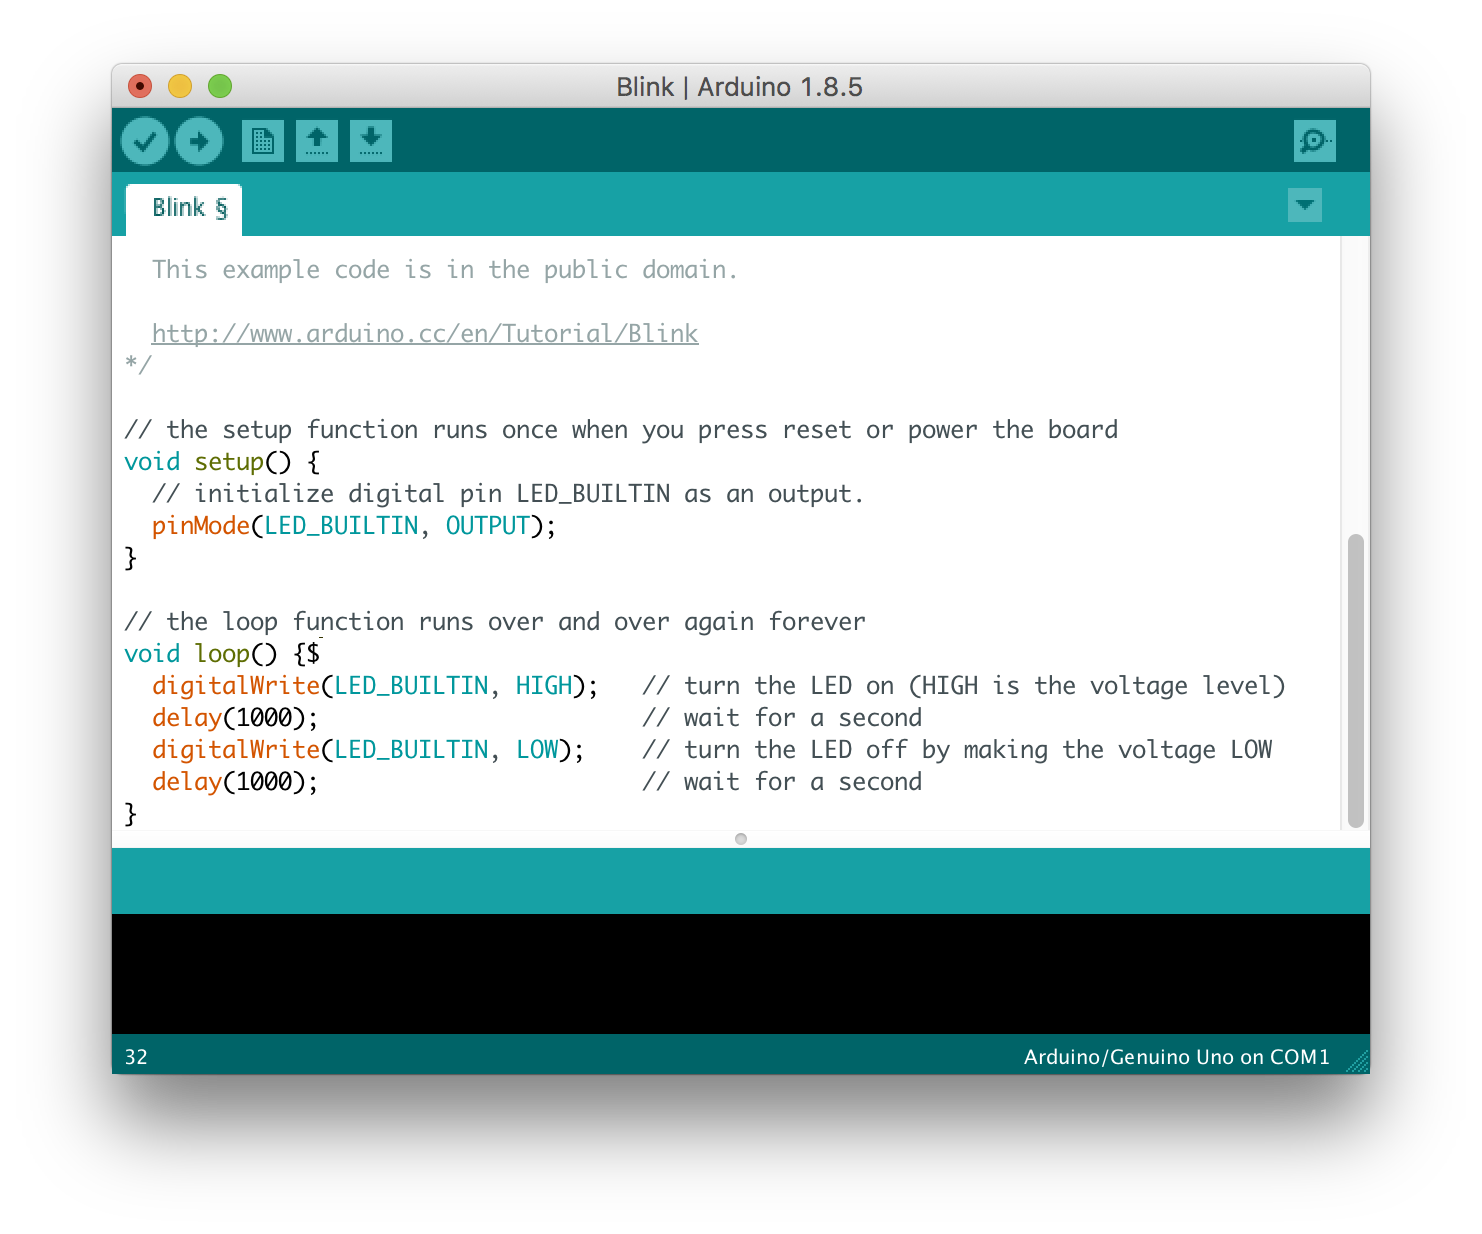
\includegraphics{images/Arduino_IDE_-_Blink.png}
\caption{\emph{Arduino IDE showing an example program (image credit: \href{https://commons.wikimedia.org/wiki/File:Arduino_IDE_-_Blink.png}{Cedar101 {[}CC0{]}, wikimedia.org})}}
\end{figure}

Part of the beauty of Arduino is its open-source nature. Many spin-offs and flavors of Arduino exist due to it's open-source nature, each with its own unique benefits. In this class, we'll use a variant of Arduino called the \textbf{\emph{Teensy}} (specifically Teensy 3.5). The Teensy is programmed in the same way as an Arduino, but has a smaller form-factor and more capabilities than a standard Arduino. The picture below shows a Teensy 3.5 and the functions of each connection on the Teensy. Seeing all the functions laid out like that can be overwhelming, but we'll walk through the ones we need to use step-by-step in future exercises.

\begin{figure}
\centering
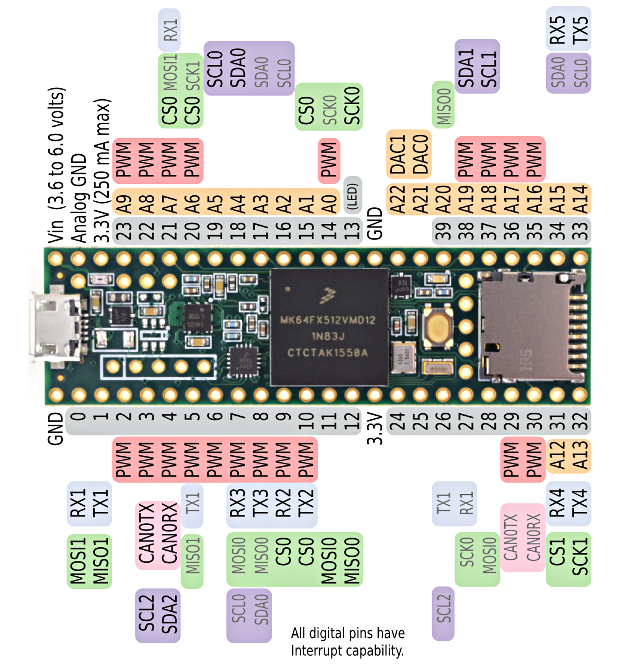
\includegraphics{images/card8a_rev2.png}
\caption{\emph{A Teensy Board, with the pin (connection) numbers and functionalities shown (reprinted from \href{https://www.pjrc.com/teensy/pinout.html}{PJRC.com}).}}
\end{figure}

This exercise will walk you through installation of the Arduino IDE, the software for the Teensy (Teensyduino), and an initial check of the board.

\hypertarget{install-the-arduino-ide}{%
\section{Install the Arduino IDE}\label{install-the-arduino-ide}}

\begin{quote}
\emph{You MUST follow the order of the instructions here or Teensyduino will not work!}
\end{quote}

\begin{enumerate}
\def\labelenumi{\arabic{enumi}.}
\tightlist
\item
  Use a web browser to navigate to \url{https://www.arduino.cc/en/Main/OldSoftwareReleases\#previous}.
\item
  Download the installer for version \textbf{1.8.6}. You must choose the installer appropriate for your operating system.
\item
  Choose \textbf{Just Download} to download the software, or make a donation if you're feeling generous!
\item
  Open the file that downloads and run the installer.
\item
  Open the Arduino program to make sure it runs and to prepare for the next steps.
\end{enumerate}

\hypertarget{install-teensyduino}{%
\section{Install Teensyduino}\label{install-teensyduino}}

\begin{enumerate}
\def\labelenumi{\arabic{enumi}.}
\tightlist
\item
  Use a web browser to navigate to \url{https://www.pjrc.com/teensy/td_download.html}.
\item
  Download the correct installer for your operatring system. Note that steps 1 and 2 on the Teensy page should have been completed when you installed the Arduino IDE, above.
\item
  Run the installer. When prompted:
\item
  Select the \texttt{Arduino/} folder for the install location. If \textbf{Next} is greyed out you probably downloaded the wrong version of the Arduino IDE.
\item
  Select \textbf{All} when asked which additional libraries to install.
\end{enumerate}

\hypertarget{test-the-teensy}{%
\section{Test the Teensy!}\label{test-the-teensy}}

\hypertarget{check-the-board}{%
\subsection{Check the board}\label{check-the-board}}

\begin{enumerate}
\def\labelenumi{\arabic{enumi}.}
\item
  Plug your Teensy into the computer via the USB connection.

  \begin{quote}
  BE \textbf{\emph{EXTREMELY}} CAREFUL WITH THE USB CONNECTION ON THE TEENSY. THEY BREAK \textbf{\emph{VERY}} EASILY!!
  \end{quote}
\item
  You should see the orange light blinking on the Teensy. If you do not, something is wrong with your Teensy and you should notify your instructor.
\end{enumerate}

\hypertarget{check-the-software}{%
\subsection{Check the software}\label{check-the-software}}

\begin{enumerate}
\def\labelenumi{\arabic{enumi}.}
\tightlist
\item
  Open the Arduino IDE.
\item
  Click \texttt{Tools\ \textgreater{}\ Board\ \textgreater{}\ Teensy\ 3.5}
\item
  Click \texttt{File\ \textgreater{}\ Examples\ \textgreater{}\ 01.Basics\ \textgreater{}\ Blink}.
\item
  Find the part in the program that says \texttt{delay(1000)} and change it to \texttt{delay(500)}.
\item
  Click \textbf{Verify} in the software (checkmark button in upper left corner).
\item
  Press the white button on the top of the Teensy.
\item
  Press upload in the software (right arrow button, next to checkmark).
\item
  You should see the orange light blink more quickly. If you encountered any errors, something could be wrong with your software installation or you may have made a typo in the code. Notify your instructor of any problems.
\end{enumerate}

\hypertarget{blink-an-led}{%
\chapter{Blink an LED}\label{blink-an-led}}

\textbf{Objective:} Use Arduino to turn an LED on and off.\\
\textbf{To turn in:} Your working Arduino code and the \href{https://github.com/alphonse/alphonse.github.io/raw/master/archive/chem191-f2019/pdf/lab2_Blink.pdf}{Lab 2 Worksheet}.

\hypertarget{introduction-1}{%
\section*{Introduction}\label{introduction-1}}
\addcontentsline{toc}{section}{Introduction}

This exercise will explore two concepts: (1) connecting devices to the Arduino and (2) the structure of the Arduino program used to \emph{control} those devices. As a first example, we'll connect an LED (light-emitting diode) to the Teensy and write a program to turn it on and off.

\hypertarget{how-are-things-connected-to-a-teensy}{%
\subsection*{How are things connected to a Teensy?}\label{how-are-things-connected-to-a-teensy}}
\addcontentsline{toc}{subsection}{How are things connected to a Teensy?}

The Teensy can control all sorts of devices, including lights, motors, and various sensors. The device to be controlled must be connected to one of the Teensy's \emph{pins}. You can think of a pin as a unique port or connection on the Teensy. Pins can send and receive information, so communication between the pin and the sensor goes both ways. One pin might be used to control a heater, while another might be used to read data from a temperature sensor. The pins that are available on the Teensy are shown in the figure below. Some pins provide power (3.3 V), some pins provide a connection to the circuit ground (GND), and some function to send and receive data. A lot of pins have several functions, each represented by a different color rectangle on the diagram. Note, though, that each pin can only have one function at any given time. For now, we'll just focus on the pin numbers. Those labeled 0-33 (shown in grey) are called \emph{digital pins}; they function as both inputs (to receive data, or sense) and outputs (send data, or control), but we'll use just the output functionality in this exercise.

\begin{figure}
\centering
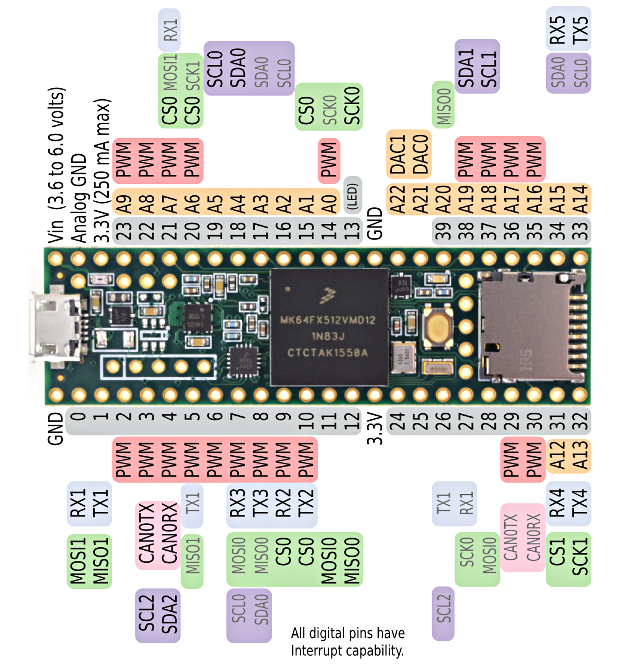
\includegraphics{images/card8a_rev2.png}
\caption{\emph{A Teensy Board, with the pin (connection) numbers and functionalities shown (reprinted from \href{https://www.pjrc.com/teensy/pinout.html}{PJRC.com}).}}
\end{figure}

There are several ways to connect something to the pins of the Teensy. One way is to directly solder wires to them, in which a soft metal alloy is melted onto two the wire and the Teensy pins as they are connected to make a permanent, metal connection. This is best saved for a final, fully vetted design that won't ever need to be changed. We'll use another method for this exercise called a solderless breadboard.

\hypertarget{the-solderless-breadboard}{%
\subsection*{The solderless breadboard}\label{the-solderless-breadboard}}
\addcontentsline{toc}{subsection}{The solderless breadboard}

A breadboard is shown in the figure below. The holes in the breadboard are spaced in such a way that a Teensy can be plugged directly into the board. Columns, labelled A, B, C, \ldots, are connected across the board electrically, such that A1 and B1 are connected; rows are insulated from each other, such that A1 and A2 are not connected. The connections labeled with red and blue lines on each edge are connected together and are sometimes called rails; they provide an easy way to distribute power (e.g.~the red rail) and ground (e.g.~the blue rail) connections around the board. If that seems confusing, try watching this video \href{https://www.youtube.com/watch?v=mLOxoK1zj9A}{this video}.

\begin{figure}
\centering
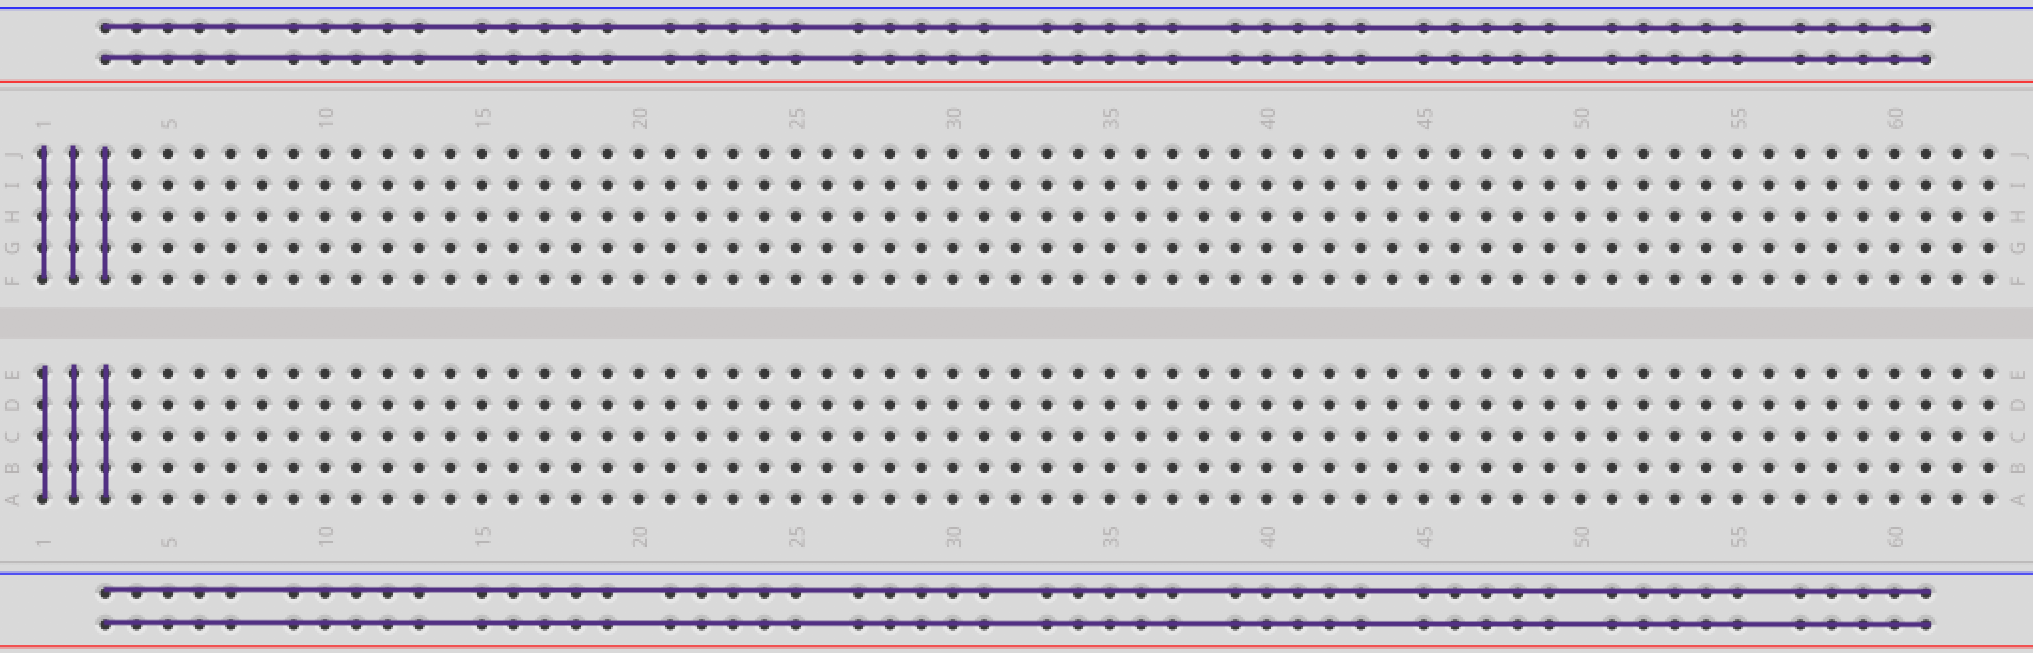
\includegraphics{images/breadboard.png}
\caption{\emph{A solderless breadboard with purple lines indicating connected holes; the pattern continues down the board. Holes with the same number are connected electrically, except across the gap in the middle, while holes with different numbers are electrically insulated.}}
\end{figure}

\hypertarget{what-is-a-program}{%
\subsection*{What is a program?}\label{what-is-a-program}}
\addcontentsline{toc}{subsection}{What is a program?}

A \emph{program}, or \emph{sketch} in Arduino jargon, is a set of commands stored on the Teensy that tell it what to do. Although a Teensy can do most anything a computer would do, it can only run a single program over and over. For example, this exercise involves programming the Teensy to turn an LED on and off so that it blinks. Other options would be to collect data from a temperature sensor, or turn a motor on a off to move a robot (or to do all of those things at once).

An Arduino program always consists of two parts: (1) a \texttt{setup()} function and (2) a \texttt{loop()} function (more details about what a function is will come in future exercises). The \texttt{setup()} function runs once every time the Teensy is powered on. After that, the Teensy runs the \texttt{loop()} function over and over until it's turned off. Usually, some initial lines of code are included above the \texttt{setup()} function provide definitions used throughout the program. A ``bare minimum'' program with the \texttt{setup()} and \texttt{loop()} functions is shown below. Note that this program does nothing other than run.

\begin{Shaded}
\begin{Highlighting}[]
    \DataTypeTok{void}\NormalTok{ setup() \{}
      \CommentTok{// anything written here will execute exactly once on startup}
\NormalTok{    \}}
    
    \DataTypeTok{void}\NormalTok{ loop() \{}
      \CommentTok{// anything written here will execute over and over indefinitely until the power is turned off}
\NormalTok{    \}}
\end{Highlighting}
\end{Shaded}

Arduino sketches (programs) are written with the Arduino IDE (see Chapter 1). To begin, you open the IDE and write your code in the text area of the program. When your're done writing your code, you compile it and upload it to the board to run it. If it compiles and uploads correctly, you will see a ``Success'' message in the message are of the IDE; if not, you'll see an error message and will need to troubleshoot your code.

You should use comments when writing your program to clairfy what each part does. Comments are not read by the compiler/board, and do not execute. In other words, they are only to help humans reading the code understand it more easily. To add a comment, just use the \texttt{\textbackslash{}\textbackslash{}} symbol; anything after that symbol won't be read by the program. For example, you can make an entire line a comment, like the first line below.

\begin{Shaded}
\begin{Highlighting}[]
    \CommentTok{// Pin 13 has the LED on Teensy 3.0}
    \DataTypeTok{int}\NormalTok{ led = }\DecValTok{13}\NormalTok{;}
\end{Highlighting}
\end{Shaded}

You could also make a portion of a line a comment, like the second half of the line below.

\begin{Shaded}
\begin{Highlighting}[]
    \DataTypeTok{int}\NormalTok{ led = }\DecValTok{13}\NormalTok{; }\CommentTok{// Pin 13 has the LED on Teensy 3.0}
\end{Highlighting}
\end{Shaded}

Finally, note that every line in the program \emph{must} end with a semi-colon, \texttt{;}.

In the exercise, we'll connect an 3-color LED to a Teensy and write a sketch to control it.

\hypertarget{connecting-the-led}{%
\section{Connecting the LED}\label{connecting-the-led}}

\begin{enumerate}
\def\labelenumi{\arabic{enumi}.}
\item
  Push your Teensy into the breadboard provided and connect the USB cable. Try not to bend the pins as you push it in. Refer to the diagram below if necessary.

  \begin{quote}
  REMEMBER, BE \textbf{\emph{EXTREMELY}} CAREFUL WITH THE USB CONNECTION ON THE TEENSY. THEY BREAK \textbf{\emph{VERY}} EASILY!!
  \end{quote}
\item
  Push the LED into the breadboard such that none of the leads (wires) are connected to anything else (each one is in it's own row). Make sure you note which row the longer lead goes into.

  \begin{quote}
  \emph{Always work with the Teensy unplugged from the computer. This will help ensure no ``magic smoke'' escapes.}
  \end{quote}
\item
  Use a jumper wire to connect the \textbf{longer lead} on the LED to the \textbf{GND} pin on the Teensy.
\item
  Use 3 more jumper wires to connect the remaining three leads to pins \textbf{13, 14, and 15}.
\end{enumerate}

\begin{figure}
\centering
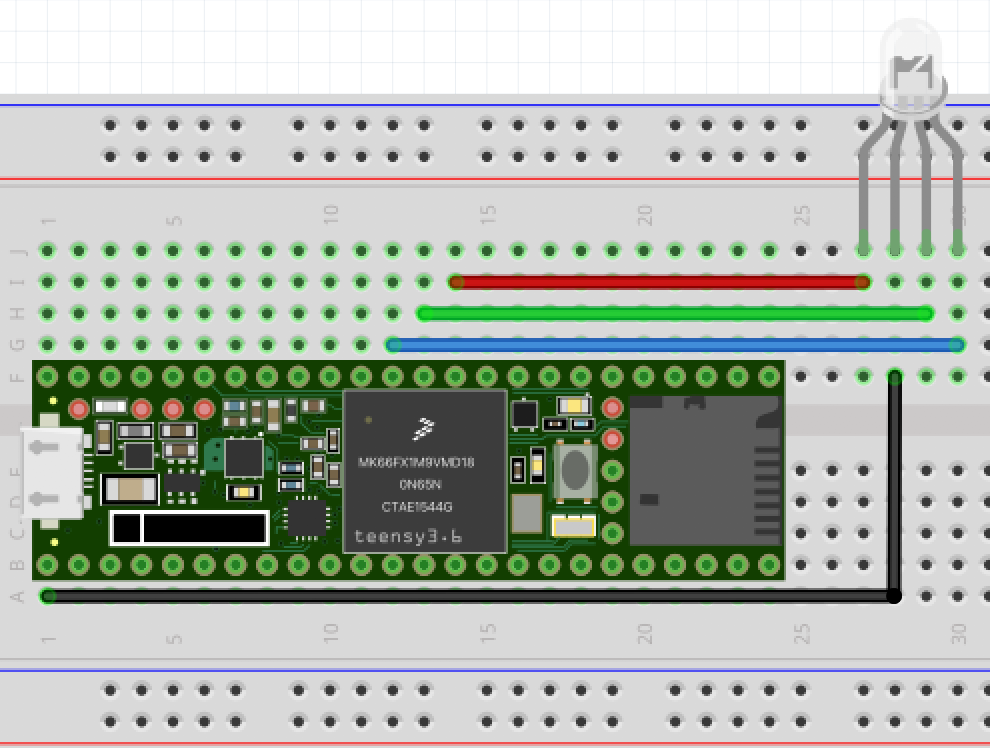
\includegraphics{images/breadboard_led_teensy.png}
\caption{\emph{Your final setup should look something like this picture.}}
\end{figure}

\hypertarget{program-the-teensy}{%
\section{Program the Teensy}\label{program-the-teensy}}

\hypertarget{one-color}{%
\subsection{One Color}\label{one-color}}

\begin{enumerate}
\def\labelenumi{\arabic{enumi}.}
\item
  Open the Arduino IDE and load the Blink example (\texttt{File\ \textgreater{}\ Examples\ \textgreater{}\ 0.1\ Basic\ \textgreater{}\ Blink})
\item
  Go to \texttt{File\ \textgreater{}\ Save\ As} to save the example under a new name in the default location (\texttt{Documents/Arduino}). Call it \textbf{lastnameFirstname\_blink.ino}.

  \begin{quote}
  \emph{Remember, files that don't follow the naming convention \textbf{exactly} will incur point deductions.}
  \end{quote}
\item
  You should see the following at the top of the sketch:
\end{enumerate}

\begin{Shaded}
\begin{Highlighting}[]
    \CommentTok{// Pin 13 has the LED on Teensy 3.0}
    \CommentTok{// give it a name:}
    \DataTypeTok{int}\NormalTok{ led = }\DecValTok{13}\NormalTok{;}
\end{Highlighting}
\end{Shaded}

Remember, anything following a \texttt{//} is a comment; it does not affect the Arduino program. Get in the habit of using comments to describe what each line of code does.

The line \texttt{int\ led\ =\ 13} defines the name of pin 13 as \texttt{led}. This name could be anything you wish. In this case, \texttt{led} is useful because the LED is connected to pin 13.

\begin{enumerate}
\def\labelenumi{\arabic{enumi}.}
\setcounter{enumi}{3}
\tightlist
\item
  Next is the \texttt{setup()} function. In this case, the only setup necessary is to set the mode of the \texttt{led} pin as an output.
\end{enumerate}

\begin{Shaded}
\begin{Highlighting}[]
  \CommentTok{// the setup routine runs once when you press reset:}
  \DataTypeTok{void}\NormalTok{ setup() \{                }
    \CommentTok{// initialize the digital pin as an output.}
\NormalTok{    pinMode(led, OUTPUT);     }
\NormalTok{  \}}
\end{Highlighting}
\end{Shaded}

\begin{enumerate}
\def\labelenumi{\arabic{enumi}.}
\setcounter{enumi}{4}
\tightlist
\item
  Finally, the \texttt{loop()} function, which runs over and over.
\end{enumerate}

\begin{Shaded}
\begin{Highlighting}[]
\NormalTok{  digitalWrite(led, HIGH);   }\CommentTok{// turn the LED on (HIGH is the voltage level)}
\NormalTok{  delay(}\DecValTok{1000}\NormalTok{);               }\CommentTok{// wait for a second}
\NormalTok{  digitalWrite(led, LOW);    }\CommentTok{// turn the LED off by making the voltage LOW}
\NormalTok{  delay(}\DecValTok{1000}\NormalTok{);               }\CommentTok{// wait for a second}
\end{Highlighting}
\end{Shaded}

\begin{enumerate}
\def\labelenumi{\arabic{enumi}.}
\setcounter{enumi}{5}
\tightlist
\item
  Assuming all those sections look good, press the \textbf{Upload} to button (right arrow in top left) to save, compile, and upload your sketch.
\end{enumerate}

\hypertarget{three-colors}{%
\subsection{Three Colors}\label{three-colors}}

You should have seen a single color blinking on and off. Now, make some modifications so that all three colors blink on and off.

\begin{enumerate}
\def\labelenumi{\arabic{enumi}.}
\tightlist
\item
  Define the two extra pins. In this case, it could be useful to refer to them by color.
\end{enumerate}

\begin{Shaded}
\begin{Highlighting}[]
    \DataTypeTok{int}\NormalTok{ blue = }\DecValTok{13}\NormalTok{;   }\CommentTok{// blue pin connected to pin 13}
    \DataTypeTok{int}\NormalTok{ green = }\DecValTok{14}\NormalTok{;  }\CommentTok{// green pin connected to pin 14}
    \DataTypeTok{int}\NormalTok{ red = }\DecValTok{15}\NormalTok{;    }\CommentTok{// red pin connected to pin 15}
\end{Highlighting}
\end{Shaded}

\begin{quote}
\emph{Have you saved your work yet? The IDE doesn't autosave, so make sure you save it \textbf{frequently}!}
\end{quote}

\begin{enumerate}
\def\labelenumi{\arabic{enumi}.}
\setcounter{enumi}{1}
\tightlist
\item
  Set each of those to outputs in the \texttt{setup()} function. You will have to fill in the blanks for the red and green pins below.
\end{enumerate}

\begin{Shaded}
\begin{Highlighting}[]
  \CommentTok{// the setup routine runs once when you press reset:}
  \DataTypeTok{void}\NormalTok{ setup() \{                }
\NormalTok{    pinMode(blue, OUTPUT);     }\CommentTok{// initialize the blue pin as an output.}
\NormalTok{    pinMode(____, OUTPUT);     }\CommentTok{// initialize the green pin as an output.}
\NormalTok{    ______________________     }\CommentTok{// initialize the red pin as an output.}
\NormalTok{  \}}
\end{Highlighting}
\end{Shaded}

\begin{enumerate}
\def\labelenumi{\arabic{enumi}.}
\setcounter{enumi}{2}
\tightlist
\item
  Finally, add the extra colors to the \texttt{loop()} function.
\end{enumerate}

\begin{Shaded}
\begin{Highlighting}[]
  \CommentTok{// blue}
\NormalTok{  digitalWrite(blue, HIGH);   }\CommentTok{// turn the LED on (HIGH is the voltage level)}
\NormalTok{  delay(}\DecValTok{1000}\NormalTok{);                }\CommentTok{// wait for a second}
\NormalTok{  digitalWrite(blue, LOW);    }\CommentTok{// turn the LED off by making the voltage LOW}
\NormalTok{  delay(}\DecValTok{1000}\NormalTok{);                }\CommentTok{// wait for a second}
  
  \CommentTok{// green}
\NormalTok{  digitalWrite(green, HIGH);   }\CommentTok{// turn the LED on (HIGH is the voltage level)}
\NormalTok{  delay(}\DecValTok{1000}\NormalTok{);                 }\CommentTok{// wait for a second}
\NormalTok{  digitalWrite(green, LOW);    }\CommentTok{// turn the LED off by making the voltage LOW}
\NormalTok{  delay(}\DecValTok{1000}\NormalTok{);                 }\CommentTok{// wait for a second}
  
  \CommentTok{// red}
\NormalTok{  digitalWrite(red, HIGH);     }\CommentTok{// turn the LED on (HIGH is the voltage level)}
\NormalTok{  delay(}\DecValTok{1000}\NormalTok{);                 }\CommentTok{// wait for a second}
\NormalTok{  digitalWrite(red, LOW);      }\CommentTok{// turn the LED off by making the voltage LOW}
\NormalTok{  delay(}\DecValTok{1000}\NormalTok{);                 }\CommentTok{// wait for a second}
\end{Highlighting}
\end{Shaded}

\begin{enumerate}
\def\labelenumi{\arabic{enumi}.}
\setcounter{enumi}{3}
\tightlist
\item
  Make sure you show your code and blinking LED to your instructor before you move on.
\end{enumerate}

\hypertarget{make-your-own-changes}{%
\subsection{Make Your Own Changes}\label{make-your-own-changes}}

\begin{enumerate}
\def\labelenumi{\arabic{enumi}.}
\tightlist
\item
  Before you leave, modify your code to change the blink pattern. You can change the sequence of the colors, the time between blinks, the number of blinks, or the amount of time each color is on.
\end{enumerate}

\hypertarget{turn-in}{%
\subsection{Turn in}\label{turn-in}}

\begin{enumerate}
\def\labelenumi{\arabic{enumi}.}
\item
  A hardcopy of your completed Exercise 2 Worksheet.
\item
  An electronic copy of your final Blink code (submit to Dropbox).

  \begin{quote}
  \emph{Remember, files that don't follow the naming convention \textbf{exactly} will incur point deductions.}
  \end{quote}
\end{enumerate}

\hypertarget{voltage-and-communication}{%
\chapter{Voltage and Communication}\label{voltage-and-communication}}

\textbf{Objective:} Measure a temperature with Teensy and display the result to the computer screen using serial communication.\\
\textbf{To turn in:}

\hypertarget{introduction-2}{%
\section*{Introduction}\label{introduction-2}}
\addcontentsline{toc}{section}{Introduction}

In the last exercise you used a Teensy to turn a light on and off, although we did not discuss what was happening electrically. This exercise will explore the electrical workings of the Teensy and walk you through how to write code to \emph{sense} signals from a device. More specifically, you'll investigate (1) the concept of \textbf{voltage} while sensing temperature and (2) communicating .

\hypertarget{electricity}{%
\subsection*{Electricity}\label{electricity}}
\addcontentsline{toc}{subsection}{Electricity}

When first learning about electricity, it may help to think of it in analogous terms to water. \textbf{Current} is the flow of electricity through a circuit, and is analogous to the current in a river. Just like water molecules move through the river, charge carriers (electrons) in a move through the wires of the circuit. \textbf{Voltage} is a \emph{potential energy difference} between two points in a circuit. This is analogous to the potential energy difference in water stored behind a dam and water at the bottom of the dam. Current will not flow without a voltage difference, just as water will not flow without a difference in height or pressure.

Recall that in the last exercise you turned an LED on and off using a pin on the Teensy. You did this by alternately setting the pin to \texttt{HIGH} and \texttt{LOW}, as in:

\begin{Shaded}
\begin{Highlighting}[]
\NormalTok{    digitalWrite(}\DecValTok{13}\NormalTok{, HIGH);}
\NormalTok{    delay(}\DecValTok{1000}\NormalTok{);}
\NormalTok{    digitalWrite(}\DecValTok{13}\NormalTok{, LOW);}
\NormalTok{    delay(}\DecValTok{1000}\NormalTok{);}
\end{Highlighting}
\end{Shaded}

But what did this do internally in the Teensy? When the Teensy gets the command \texttt{digitalWrite(13,\ HIGH);} it sets the voltage of pin 13 to 3.3 volts (3.3 V is standard voltage for microcontrollers). Alternatively, when it gets the command \texttt{digitalWrite(13,\ LOW);}, it sets the voltage to 0 V. Thus, when the voltage is 3.3 V, there is a potential difference across the LED from 3.3 V on the controlling pin (anode) to 0V on the ground pin (cathode). This causes current to flow through the LED, which in turn causes the LED to light up. When the voltage is set back to 0, there is no longer a potential difference across the LED, current does not flow, and the LED does not light up.

You may have gotten the idea that voltage and current are inextricably linked, and that's true. In fact, \textbf{Ohm's Law} provides a mathmatical relation between the two:

\[
\text{Voltage (volts)} = \text{Current (amps)} \times \text{Resistance (ohms, }\Omega\text{)}  \\
V = iR
\]

This introduces a new concept, resistance. \textbf{Resistance} is simply the opposition to flow of electrical current. Resistance can be introduced to a circuit purposely with a device called a \textbf{resistor}. Usually these are a defined, fixed resistance introduced for a specific purpose. However, many sensors have a resistance that changes proporitionally to some stimulus. Thus, the voltage across the device will change in response to that stimulus, and the stimulus can be measured simply by measuring the voltage. As an example of how useful this is, consider a temperature sensor. A computer or microcontroller cannot sense the temperature directly -- it only understands voltages. A device that converts changes in temperature to changes in voltage allows the computer to infer changes in temperature.

Although the voltage output from the Teensy pin was either HIGH or LOW, the voltage output from the temperature sensor can be any value. A signal that can be only HIGH or LOW (i.e.~on or off, 1 or 0), is called a \textbf{digital signal}. Digital signals are often used to communicate between computers and to control many devices because they are relatively immune to outside noise. Many sensors, on the other hand, produce signals that vary \emph{continuously}, and such signals are called \textbf{analog signals}.

The Teensy can read \emph{digital} signals on any of its digital I/O (input/output) pins (grey labels on the pinout diagram). The Teensy can read \emph{analog} signals on any of the analog input pin, which are shown with orange labels in the pinout diagram and numbered A0 through A22 (the A stands for analog).

\hypertarget{bits-and-volts}{%
\subsection*{Bits and Volts}\label{bits-and-volts}}
\addcontentsline{toc}{subsection}{Bits and Volts}

Even though Teensy can ``read'' analog signals, it only understands digital signals. So every analog signal read by the Teensy gets sent through an \emph{analog to digital converter} (ADC). This converts the analog signal from a sensor into a digital signal with discrete steps. The size of these steps is determined by the number of \textbf{bits} the ADC has. More bits equals more steps, and more steps equals a digital signal that more closely approximates the real analog signal.

\hypertarget{communicating-via-the-serial-port}{%
\subsection*{Communicating via the serial port}\label{communicating-via-the-serial-port}}
\addcontentsline{toc}{subsection}{Communicating via the serial port}

In the previous exercise, you used digital signals to control an LED, but there was no communication between the Teensy and computer after the sketch was uploaded. When reading signals, it's often useful to display the reading on the computer screen to have real-time feedback from the program. To do this, the data collected on the Teensy board must be sent to the computer, the computer must read the data, and the computer must display it on the screen. The communication protocol used to do this is called \textbf{serial communication}. This is a very widely used protocol, and most computers used to come with a serial port built in. In our case, we'll conduct serial communication over the USB port.

Using serial communication on the Teensy is relatively simple. The first step is to open the serial port and tell it what data transfer speed to use (basically how quickly the Teensy and the computer talk to each other).

\begin{Shaded}
\begin{Highlighting}[]
\NormalTok{    Serial.begin(}\DecValTok{9600}\NormalTok{);}
\end{Highlighting}
\end{Shaded}

Once the connection is open, you can print most anything to the serial port you wish. For example, a simple \href{https://en.wikipedia.org/wiki/\%22Hello,_World!\%22_program}{hello world} program would look something like:

\begin{Shaded}
\begin{Highlighting}[]
\NormalTok{    Serial.begin(}\DecValTok{9600}\NormalTok{);}
\NormalTok{    Serial.print(}\StringTok{"Hello, World!"}\NormalTok{);}
\end{Highlighting}
\end{Shaded}

The above pseudocode would print ``Hello, World!'' to the computer's serial port. The result could be displayed on the computer screen by opening the serial monitor in the Arduino IDE. There are a few more details you'll learn as you go.

In this exercise, you'll measure ambient temperatures using a temperature sensor and display the result to the computer screen via the serial port.

\hypertarget{connect-the-temperature-sensor}{%
\section{Connect the Temperature Sensor}\label{connect-the-temperature-sensor}}

\begin{enumerate}
\def\labelenumi{\arabic{enumi}.}
\item
  Push your Teensy into the breadboard provided and connect the USB cable. Try not to bend the pins as you push it in. Refer to the diagram below if necessary.

  \begin{quote}
  REMEMBER, BE \textbf{\emph{EXTREMELY}} CAREFUL WITH THE USB CONNECTION ON THE TEENSY. THEY BREAK \textbf{\emph{VERY}} EASILY!!
  \end{quote}
\item
  Push the sensor into the breadboard such that neither of the leads (wires) are connected to anything else (each one is in it's own row). The orientation does not matter; both legs are the same.

  \begin{quote}
  \emph{Always work with the Teensy unplugged from the computer. This will help ensure no ``magic smoke'' escapes.}
  \end{quote}
\item
  Use a jumper wire to connect one side of the sensor to Vin/5V on the Teensy (side 1).
\item
  Connect the other side (side 2) of the sensor to a 10 kilo-ohm (k\(\\Ohm\)) resistor, and then connect the other side of the resistor to ground (GND on the Teensy). You may need to use a jumper wire to connect the resistor to GND.
\item
  Use a jumper wire to connect side 2 of the sensor to an analog input on the Teensy. In the example below, pin A0 is used.
\end{enumerate}

\begin{figure}
\centering
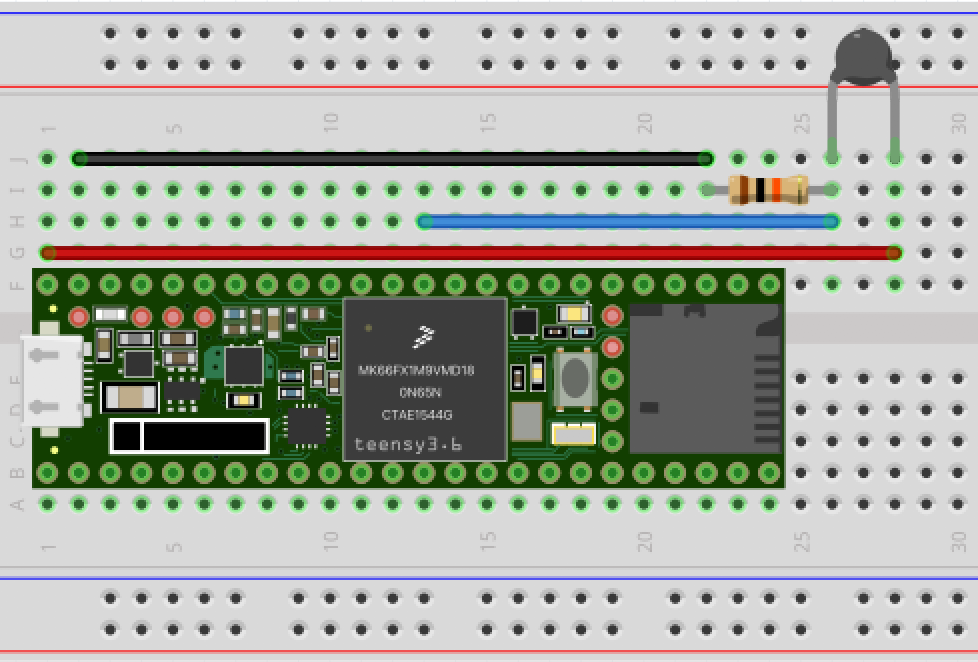
\includegraphics{images/breadboard_thermistor_teensy.png}
\caption{\emph{Your final setup should look something like this picture. Red = 5V, black = GND, and blue = signal. }}
\end{figure}

\hypertarget{program-the-teensy-1}{%
\section{Program the Teensy}\label{program-the-teensy-1}}

\hypertarget{bare-minimum}{%
\subsection{Bare Minimum}\label{bare-minimum}}

\begin{enumerate}
\def\labelenumi{\arabic{enumi}.}
\item
  Open the Arduino IDE and load a new file (if one doesn't open automatically).
\item
  Go to \texttt{File\ \textgreater{}\ Save\ As} to save the example under a new name in the default location (\texttt{Documents/Arduino}). Call it \textbf{groupName\_voltage.ino}.

  \begin{quote}
  \emph{Remember, files that don't follow the naming convention \textbf{exactly} will incur point deductions.}
  \end{quote}
\item
  Create a \texttt{setup()} function and start serial communication within it:
\end{enumerate}

\begin{Shaded}
\begin{Highlighting}[]
    \DataTypeTok{void}\NormalTok{ setup() \{}
\NormalTok{        Serial.begin(}\DecValTok{9600}\NormalTok{);  }\CommentTok{// start serial communication at a rate of 9600 bits per second (the standard)}
\NormalTok{    \}}
\end{Highlighting}
\end{Shaded}

\begin{enumerate}
\def\labelenumi{\arabic{enumi}.}
\setcounter{enumi}{3}
\tightlist
\item
  Create a \texttt{loop()} function, read the sensor data, and print it to the serial port:
\end{enumerate}

\begin{Shaded}
\begin{Highlighting}[]
    \DataTypeTok{void}\NormalTok{ loop() \{}
\NormalTok{        value = analogRead(}\DecValTok{0}\NormalTok{); }\CommentTok{// read sensor}
\NormalTok{        Serial.println(value); }\CommentTok{// print result to serial port}
\NormalTok{        delay(}\DecValTok{1000}\NormalTok{);           }\CommentTok{// wait for 1 second}
\NormalTok{    \}}
\end{Highlighting}
\end{Shaded}

\begin{enumerate}
\def\labelenumi{\arabic{enumi}.}
\setcounter{enumi}{4}
\tightlist
\item
  Press the \textbf{Upload} button to send your sketch to the Teensy. Once you get it loaded, click the \textbf{Serial Monitor} button to see if the communication is working. You should see a number between 400 and 500 if you sensor is working correctly.
\end{enumerate}

\hypertarget{converting-to-temperature}{%
\subsection{Converting to Temperature}\label{converting-to-temperature}}

The Teensy reports values in bits, which isn't very meaningful to humans. What we really care about is the temperature. The formula to get from bits to degrees C (for this sensor connected to a Teensy) is:

\begin{verbatim}
$$
    ^{\circ}C = 25 + (\text{value} - 512) / 11.3
$$
\end{verbatim}

\begin{enumerate}
\def\labelenumi{\arabic{enumi}.}
\tightlist
\item
  Add the above forumla to your code to convert to temperature. Also change the code to print the temperature to the serial port instead of the raw value.
\end{enumerate}

\begin{Shaded}
\begin{Highlighting}[]
    \DataTypeTok{void}\NormalTok{ loop() \{}
\NormalTok{        value = analogRead(}\DecValTok{0}\NormalTok{); }\CommentTok{// read sensor}
\NormalTok{        temp  = ____________________________; }\CommentTok{// convert to temperature}
\NormalTok{        ______________________; }\CommentTok{// print the temperature to the serial port.}
\NormalTok{        delay(}\DecValTok{1000}\NormalTok{);            }\CommentTok{// wait for 1 second}
\NormalTok{    \}}
\end{Highlighting}
\end{Shaded}

\begin{enumerate}
\def\labelenumi{\arabic{enumi}.}
\tightlist
\item
  Upload your code and see if it works.
\end{enumerate}

\hypertarget{cleaning-up-the-output}{%
\subsection{Cleaning up the Output}\label{cleaning-up-the-output}}

You can also print text to the serial port. When you use \texttt{Serial.print()} or \texttt{Serial.println()} to print text, it should always be in quote marks (this is technically called a \emph{string}). For example, \texttt{Serial.println(Hello,\ world!)} would NOT work, but \texttt{Serial.println("Hello,\ world!")} would. To clean up you data output, try printing "*C" after the temperature to indicate the units.

\begin{enumerate}
\def\labelenumi{\arabic{enumi}.}
\tightlist
\item
  Change \texttt{Serial.println(temp)} to \texttt{Serial.print(temp)}. These two functions are very similar, with one difference: \texttt{println} creates a new line when it's finished (like pressing enter on the keyboard) whereas \texttt{print} does not.
\item
  Add a line just below \texttt{Serial.print(temp)} to print the "*C" symbology:
\end{enumerate}

\begin{Shaded}
\begin{Highlighting}[]
\NormalTok{    Serial.print(temp);}
\NormalTok{    Serial.println(}\StringTok{"*C"}\NormalTok{);}
\end{Highlighting}
\end{Shaded}

\hypertarget{make-your-own-changes-1}{%
\subsection{Make Your Own Changes}\label{make-your-own-changes-1}}

\begin{enumerate}
\def\labelenumi{\arabic{enumi}.}
\tightlist
\item
  Before you leave, add a line in your code to convert from degrees C to degrees F.
\item
  Once you've converted to F, print the results for both degrees C and degrees F. Your values should:

  \begin{itemize}
  \tightlist
  \item
    Be printed to the serial port \emph{on the same line}.
  \item
    Include the units ``\emph{C" and "}F'' where needed.
  \item
    Be separated from each other with a space (either " " or `s').
  \end{itemize}
\end{enumerate}

\hypertarget{turn-in-1}{%
\subsection{Turn in}\label{turn-in-1}}

\begin{enumerate}
\def\labelenumi{\arabic{enumi}.}
\item
  A hardcopy of your completed Exercise 3 Worksheet.
\item
  An electronic copy of your final Voltage code (submit to Dropbox).

  \begin{quote}
  \emph{Remember, files that don't follow the naming convention \textbf{exactly} will incur point deductions.}
  \end{quote}
\end{enumerate}

\hypertarget{functions-building-blocks-for-programs}{%
\chapter{Functions: Building Blocks for Programs}\label{functions-building-blocks-for-programs}}

\textbf{Objective:} Create a \texttt{blink()} function in Arduino.

\hypertarget{introduction-3}{%
\section*{Introduction}\label{introduction-3}}
\addcontentsline{toc}{section}{Introduction}

In previous exercises discussed the two function, \texttt{setup()} and \texttt{loop()} that are necessary for every Arduino sketch. You've also (perhaps unknowingly) used pre-defined functions to achieve tasks. In programming, a \textbf{function} is a defined piece of reusable code that can be used to perform an action. You could think of functions as modules that can be stacked together to create a program. For example, the items \texttt{digitalWrite()} and \texttt{Serial.print()} are both functions. The first, as we've seen, controls the logic level of a digital I/O pin on the Teensy while the latter prints data to the serial port.

Note that functions all have a defined stucture, or \emph{syntax}. This may vary from language to langages, but will be the same within any language. In Arduino (C), functions always take the form \texttt{function(argument\_1,\ argument\ 2,\ ...);}, where \texttt{function()} is the function and \texttt{argument\_1}, etc., are the entities the function acts on or uses in some way while executing the function. This is very similar to functions in mathmatics. Assume, for example:

\[
f(x) = 3x \\
\]

Here, we've defined a function, \(f\), that acts on argument \(x\). If we write \(f(2)\), we are saying we wish to substitute 2 for x in the function, yielding \(f(x) = 3 \times 2 = 6\).

We could just as easily do this in Arduino. Using the same example, we can define a function \texttt{f()}:

\begin{Shaded}
\begin{Highlighting}[]
  \DataTypeTok{int}\NormalTok{ f(}\DataTypeTok{int}\NormalTok{ x) \{}
    \ControlFlowTok{return} \DecValTok{3}\NormalTok{*x}
\NormalTok{  \}}
\end{Highlighting}
\end{Shaded}

This function is equivalent to the mathmatical expression above. First, we define a function \texttt{f()} that takes one argument, \texttt{x} (contained within the parentheses). Within the function (denoted by the curly braces), we ask Arduino to output, or \textbf{return}, \(3 \times x\). After defining the function, we could write \texttt{f(2)} and Arduino would output \texttt{6}.

\begin{quote}
*What would Arduino output if you wrote \texttt{f(4)}?
\end{quote}

\hypertarget{using-functions}{%
\subsection{Using Functions}\label{using-functions}}

Although most of the work done in this class will rely on pre-written functions, You'll explore the methods for writing your own function in this exercise to help you understand how they work. As mentioned above, you can think of function as modules or building blocks that can be combined to create desired outcome. For example, if you wished to create a program that flashed a light everytime the temperature was read and then displayed the result to the screen, you might wish to combine blocks for reading the temperature, flashing a light, and printing data to the computer screen:

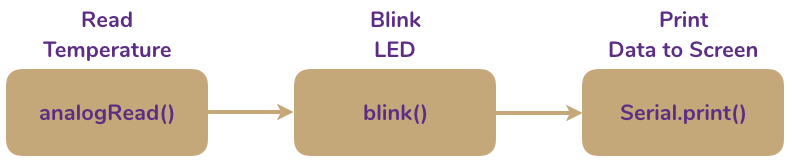
\includegraphics{images/blockDiagram_basic.png}

Creating the \textbf{block diagrams} can be very helpful in visualizing what a program will do, and just the process of creating one can help you think through what the program needs to achieve line-by-line. The program above has one problem: it assumes there is a function called \texttt{blink()} that will flash the LED. This is not true, but you'll make one in this exercise. A list of built in functions can be found on the \href{https://www.arduino.cc/reference/en/}{Arduino website}; other functions specific to this class can be found in {[}Appendix C{]}{[}Appendix C: Functions{]}.

\hypertarget{writing-a-blink-function}{%
\section{\texorpdfstring{Writing a \texttt{blink()} Function}{Writing a blink() Function}}\label{writing-a-blink-function}}

\begin{enumerate}
\def\labelenumi{\arabic{enumi}.}
\tightlist
\item
  On your worksheet, create a diagram like the one above for a function that would blink and LED on and off. Your function should:
\end{enumerate}

\begin{itemize}
\tightlist
\item
  Be called \texttt{blink()}.
\item
  Turn the LED on for a set amount of time.
\item
  Turn the LED off for a set amount of time.
\end{itemize}

\begin{enumerate}
\def\labelenumi{\arabic{enumi}.}
\setcounter{enumi}{1}
\tightlist
\item
  Define your function in Arduino. Open a blank sketch by clicking \texttt{File\ \textgreater{}\ Examples\ \textgreater{}\ Bare\ Minimum}. Add your variable definitions to the top and set the appropriate pins as outputs in your \texttt{setup()} function using \texttt{pinMode}. Refer to your previous exercises if you can't remember how to do those things.
\end{enumerate}

\begin{Shaded}
\begin{Highlighting}[]
  \CommentTok{// define variables here}
  
  \DataTypeTok{void}\NormalTok{ setup() \{}
    \CommentTok{// set pinMode() here}
\NormalTok{  \}}
  
  \DataTypeTok{void}\NormalTok{ loop() \{}
    \CommentTok{// leave blank for now}
\NormalTok{  \}}
\end{Highlighting}
\end{Shaded}

\begin{enumerate}
\def\labelenumi{\arabic{enumi}.}
\setcounter{enumi}{2}
\tightlist
\item
  Define your \texttt{blink()} function at the bottom of your sketch. Follow the format below (don't worry about the \texttt{void} part now -- just know that you need to use it).
\end{enumerate}

\begin{Shaded}
\begin{Highlighting}[]
  \CommentTok{// define variables here}
  
  \DataTypeTok{void}\NormalTok{ setup() \{}
    \CommentTok{// set pinMode() here}
\NormalTok{  \}}
  
  \DataTypeTok{void}\NormalTok{ loop() \{}
    \CommentTok{// leave blank for now}
\NormalTok{  \}}
  
  \DataTypeTok{void}\NormalTok{ blink(}\DataTypeTok{int}\NormalTok{ ledPin) \{}
\NormalTok{    digitalWrite(ledPin, HIGH); }\CommentTok{// turn LED on}
\NormalTok{    ___________________________ }\CommentTok{// wait x milliseconds}
\NormalTok{    ___________________________ }\CommentTok{// turn LED off}
\NormalTok{    ___________________________ }\CommentTok{// wait x milliseconds}
\NormalTok{  \}}
\end{Highlighting}
\end{Shaded}

\hypertarget{using-functions-1}{%
\section{Using Functions}\label{using-functions-1}}

\begin{enumerate}
\def\labelenumi{\arabic{enumi}.}
\tightlist
\item
  Add the function into your code and test it out.
\end{enumerate}

\begin{Shaded}
\begin{Highlighting}[]
  \CommentTok{// define variables here}
  
  \DataTypeTok{void}\NormalTok{ setup() \{}
    \CommentTok{// set pinMode() here}
\NormalTok{  \}}
  
  \DataTypeTok{void}\NormalTok{ loop() \{}
\NormalTok{    blink(________);}
\NormalTok{  \}}
  
  \DataTypeTok{void}\NormalTok{ blink(}\DataTypeTok{int}\NormalTok{ ledPin) \{}
\NormalTok{    digitalWrite(ledPin, HIGH); }\CommentTok{// turn LED on}
\NormalTok{    ___________________________ }\CommentTok{// wait x milliseconds}
\NormalTok{    ___________________________ }\CommentTok{// turn LED off}
\NormalTok{    ___________________________ }\CommentTok{// wait x milliseconds}
\NormalTok{  \}}
\end{Highlighting}
\end{Shaded}

\hypertarget{write-functions-with-multiple-arguments}{%
\section{Write Functions With Multiple Arguments}\label{write-functions-with-multiple-arguments}}

\begin{enumerate}
\def\labelenumi{\arabic{enumi}.}
\tightlist
\item
  Create a second function called \texttt{blink2();}. It should do the same thing as blink but allow for a variable blinking time.
\end{enumerate}

\begin{Shaded}
\begin{Highlighting}[]
  \DataTypeTok{void}\NormalTok{ blink(}\DataTypeTok{int}\NormalTok{ ledPin, }\DataTypeTok{int}\NormalTok{ interval) \{}
    \CommentTok{// turn LED on}
    \CommentTok{// wait x milliseconds}
    \CommentTok{// turn LED off}
    \CommentTok{// wait x milliseconds}
\NormalTok{  \}}
\end{Highlighting}
\end{Shaded}

\begin{enumerate}
\def\labelenumi{\arabic{enumi}.}
\setcounter{enumi}{1}
\tightlist
\item
  Add this to your code and use it with \texttt{blink()}.
\end{enumerate}

\hypertarget{turn-in-2}{%
\section{Turn In}\label{turn-in-2}}

\begin{enumerate}
\def\labelenumi{\arabic{enumi}.}
\tightlist
\item
  Turn in a hardcopy of your completed worksheet.
\item
  Turn in an electronic copy of your code containing the functions \texttt{blink();} and \texttt{blink2()} that shows use of both.
\end{enumerate}

\hypertarget{soldering-and-pcb-assembly}{%
\chapter{Soldering and PCB Assembly}\label{soldering-and-pcb-assembly}}

\textbf{Objective:} Assemble/solder air quality sensor printed circuit board.

\hypertarget{introduction-4}{%
\section{Introduction}\label{introduction-4}}

Up to this point, we've used solderless breadboards and jumper wires to connect things to the Teensy. Those provide quick, temporary connections that can be used for prototyping and learning. However, they can be prone to failure over time as the connections inadvertently come loose. In situations where a design won't change, metal solder joints provide a more reliable, permanent connection.

Although soldering seems difficult to many people, it's actually a simple process if you have the correct tools and know the right technique. Hand soldering has been done on an industrial scale by assembly technicians for decades, and modern electronics with very small components are usually soldered by machine. In short, the soldering process involves heating up two metal parts to be joined with a \emph{soldering iron}, applying a compound called \emph{flux} to the joint, and then melting a soft metal alloy (the \emph{solder}) onto the joint. Once the solder cools (after a second or two), a permanent connection is made between the two components.

\begin{quote}
Good soldering technique, contrary to popular belief, is not hard. In fact, it's incredibly easy!

If you've got the right tools and now the very simple, basic techniques, good soldering is a piece of cake! Anyone can do it, straight up!
-\emph{Dave Jones, EEVBlog}
\end{quote}

This exercise will walk you through the basics of soldering, and by the end you should have completed assembly of your air sensor printed circuit board (PCB). The following video tutorials may be helpful in knowing what to expect before you come to class. Please watch the beginner tutorial, and then watch the longer tutorials by the EEVBlog if you would like to learn more details.

\begin{itemize}
\tightlist
\item
  \href{https://www.youtube.com/watch?v=Qps9woUGkvI}{Beginner tutorial}
\item
  In depth tutorial @ EEVBlog:

  \begin{enumerate}
  \def\labelenumi{\arabic{enumi}.}
  \tightlist
  \item
    \href{https://www.youtube.com/watch?v=J5Sb21qbpEQ}{Tools}
  \item
    \href{https://www.youtube.com/watch?v=fYz5nIHH0iY}{Through-hole Soldering}
  \item
    \href{https://www.youtube.com/watch?v=b9FC9fAlfQE}{Surface-mount Soldering}
  \end{enumerate}
\item
  schematic diagrams
\end{itemize}

\hypertarget{soldering-basics}{%
\section{Soldering Basics}\label{soldering-basics}}

\hypertarget{the-supplies}{%
\subsection{The Supplies}\label{the-supplies}}

Good tools and supplies can really make or break a soldering project. The two most important things are the solder and the soldering iron, but there are a host of other supplies that can help out.

\begin{itemize}
\tightlist
\item
  \textbf{Solder} is traditionally made from a lead alloy, although many modern solders are lead free due to the toxic nature of lead. For most hobby applications, either option will work. Solder comes in many different sizes, but in general narrower solder (\textless0.5 mm diameter) is better for electronics work. Many solders come with rosin (basically pin sap) embedded in the core, which acts as \emph{flux} and eliminates the need for pre-application of flux (described below).
\item
  \textbf{Flux} is a special compound that removes oxidation from the surface of the metals to be joined. Many metal (including copper, which is what we are soldering) form oxide layers on the surface of the metal. Although these are often difficult to see, they are always there. They will prohibit the solder from \emph{wetting} (flowing onto and adhereing to) the items to be joined. It is usually very difficult or impossible to solder a joing without flux, and joints made with it will eventually crack and fail. Many solders come with flux (rosin) embedded in the middle of the solder to act as a flux; with these solders no additional flux is necessary. Any residue left from flux can be cleaned up with isopropyl (rubbing) alcohol or special flux cleaner.
\item
  A \textbf{Soldering iron} is a pen-shaped device with a fine metal tip that is heated, usually with an electric heating element. It's always best to invest in a temperature-controlled soldering iron and skip the cheaper ones -- the proper temperature is important for good soldering. A good soldering iron should also have a removable/interchangeable tip and a safety stand to prevent fires.
\item
  A \textbf{sponge} is just a regular kitchen sponge that is dampened with water and used to clean the tip of the soldering iron during use. Keeping the tip clean helps the solder melt easily. As an alternative, a \textbf{brass sponge} (think of a metal kitchen scrubbie) can be used.
\item
  A \textbf{third hand} is just a metal stand with clips on it to hold your workpiece while you solder to it. Tape, sticky tack, and other items can be used as well.
\item
  \textbf{Flush side cutters, wire cutters, and/or wire strippers} are useful for trimming leads after they've been soldered and stripping wires prior to soldering.
\item
  \textbf{Isopropyl alcohol} or \textbf{flux remover} and a small brush are useful in removing stick residue left by the flux.
\item
  \textbf{Solder wick} and a \textbf{solder sucker} are tools used to remove solder when necessary. (Even though it said solder is ``permanent'' above, it can be removed, albeit not always in an easy manner!)
\item
  A \textbf{Fume extractor} collects the smoke released during soldering and prevents it from being breathed in by the solderer.
\end{itemize}

\hypertarget{the-technique}{%
\subsection{The Technique}\label{the-technique}}

The main thing to remember when soldering is to use heat and wettability to determine where the solder will end up. If you want solder on one part of a circuit board and not another, make sure you apply the heat and flux to that part to be soldered and no where else; the solder will folow dutifully.

\textbf{Setup}

\begin{enumerate}
\def\labelenumi{\arabic{enumi}.}
\tightlist
\item
  Check for the recommended iron temperature for the solder you're using. If you're unsure, 350\(^\circ\)C is a good starting point. If your part to be soldered is very large or you're soldering to a ground plane with a large thermal mass you made need to increase the temperature.
\item
  Turn on the soldering iron to the correct temperature.
\item
  Wet the sponge on the soldering iron stand.
\item
  Layout all the tools necessary.
\item
  Turn on the fume extractor.
\end{enumerate}

\textbf{Soldering}

\begin{enumerate}
\def\labelenumi{\arabic{enumi}.}
\tightlist
\item
  \textbf{Create a mechanical connection if possible.} If joining two wires, twist them together. If connecting a component to a circuit board, bend the leads down to hold in the place. The mechanical connection is not strictly necessary, but it will add stregnth to the solder joint.
\item
  \textbf{Stabilize the parts to be soldered.} It takes two hands to solder -- one to hold the soldering iron and one to apply the solder. Make sure your workpiece is secure before you being soldering.
\item
  {[}\textbf{Apply flux (if not using rosin-core solder).} Apply a small amount only to the parts to be soldered. Remember, the solder will folow the flux.{]}
\item
  \textbf{Clean the tip of the iron.} The soldering iron tip will develop an oxide layer as it sits at high temperature. Give a one or two wipes across the wet sponge each time you pick it up.
\item
  \textbf{Tin the tip of the iron.} Just barely touch the tip of the iron
\item
  \textbf{Apply heat to the joint.} Try to maxmize contact between the tip of the iron and the joint to be soldered. Apply heat to the solder joint, not the solder. This ensures the joint is hot enough to flow the solder and helps create a strong joint.
\item
  \textbf{Apply solder to the joint.} Touch the end of the solder to the joint to be soldered. If the joint is hot enough the solder should flow immediately throughout the joint.
\item
  \textbf{Let it cool.} Remove the solder, then the iron, and let the joint cool for a second or two before moving it. Wait longer before touching the joint as it will be hot enough to burn you.
\item
  \textbf{Inspect the joint.} A properly soldered joint should have a shiny, domed appearance. An improperly soldered joint will appear dull and blobby. Remove solder if necessary and repeat until a good joint is achieved.
\end{enumerate}

\hypertarget{safety}{%
\subsection{Safety}\label{safety}}

\begin{itemize}
\tightlist
\item
  Obviously, the soldering iron and anything it touches are hot. Don't touch the tip of the iron or any of the parts that have recently been soldered.
\item
  Always be mindful of where you set the iron down. It's hot enough to start fires and/or melt work surfaces and power cords.
\item
  Don't breath in the fumes. They mostly result from the flux. Use a fume extractor or a fume hood to keep the fumes out of your lungs!
\end{itemize}

\hypertarget{assembling-the-board}{%
\section{Assembling the Board}\label{assembling-the-board}}

You will add components to a printed circuit board (PCB) to build the air sensor. The PCB has internal connections that ensure all components will be connected correctly. The purple areas of the board are called \emph{solder mask}. Solder strongly prefers to stick to metal and will (almost) not stick to the solder mask. Use this to your advantage!

\begin{enumerate}
\def\labelenumi{\arabic{enumi}.}
\tightlist
\item
  Solder each component on one at a time. Remember to consider which ones you need to solder first and which ones last, as some components may make it hard to get the iron into areas of the PCB.
\item
  Each component is labelled on the board. Refer to the model at the front of the room if you're unsure where something goes.
\item
  Make sure your have the component in the right place and the right orientation before making the solder connection! You may not be able to remove it if you do it incorrectly!!
\end{enumerate}

\hypertarget{appendix-a-function-library}{%
\chapter*{Appendix A: Function Library}\label{appendix-a-function-library}}
\addcontentsline{toc}{chapter}{Appendix A: Function Library}

\hypertarget{blink}{%
\section*{blink()}\label{blink}}
\addcontentsline{toc}{section}{blink()}

Blinks the Teensy's onboard LED.

\begin{Shaded}
\begin{Highlighting}[]
\DataTypeTok{void}\NormalTok{ blink() \{}
\NormalTok{    digitalWriteFast(LED_BUILTIN, HIGH);}
\NormalTok{    delay(}\DecValTok{15}\NormalTok{);}
\NormalTok{    digitalWriteFast(LED_BUILTIN, LOW);}
\NormalTok{    delay(}\DecValTok{15}\NormalTok{);}
\NormalTok{\}}
\end{Highlighting}
\end{Shaded}

\hypertarget{checkconnection}{%
\section*{checkConnection()}\label{checkconnection}}
\addcontentsline{toc}{section}{checkConnection()}

Checks serial connection to PM sensor and connection to SD card and returns 5 and 2 LED blinks, respectively, if successful.

\begin{Shaded}
\begin{Highlighting}[]
\DataTypeTok{void}\NormalTok{ checkConnection() \{}
  \ControlFlowTok{if}\NormalTok{ (my_status == }\DecValTok{1}\NormalTok{)\{}
    \ControlFlowTok{for}\NormalTok{ (}\DataTypeTok{int}\NormalTok{ i = }\DecValTok{1}\NormalTok{; i < }\DecValTok{6}\NormalTok{; i++)\{}
\NormalTok{      blink();}
\NormalTok{    \}}
    
\NormalTok{    delay(}\DecValTok{3000}\NormalTok{);}
\NormalTok{  \}}
  \ControlFlowTok{else}\NormalTok{\{}
\NormalTok{    digitalWrite(LED_BUILTIN, HIGH);}
\NormalTok{    delay(}\DecValTok{5000}\NormalTok{);  }
\NormalTok{    digitalWrite(LED_BUILTIN, LOW);}
\NormalTok{  \}}

   \ControlFlowTok{if}\NormalTok{ (!SD.begin(chipSelect)) \{}
    \ControlFlowTok{return}\NormalTok{;}
\NormalTok{  \}}
  \ControlFlowTok{if}\NormalTok{ (!card.init(SPI_HALF_SPEED, chipSelect)) \{}
        \CommentTok{// don't do anything more:}
        \ControlFlowTok{while}\NormalTok{ (}\DecValTok{1}\NormalTok{) \{}
\NormalTok{            blink();}
\NormalTok{            blink();}
\NormalTok{        \}}
\NormalTok{    \}}
    \ControlFlowTok{for}\NormalTok{ (}\DataTypeTok{int}\NormalTok{ i = }\DecValTok{1}\NormalTok{; i < }\DecValTok{3}\NormalTok{; i++)\{}
\NormalTok{      blink();}
\NormalTok{    \}}
\NormalTok{\}}
\end{Highlighting}
\end{Shaded}

\hypertarget{createfilenameint-y-int-m-int-d}{%
\section*{createFileName(int y, int m, int d)}\label{createfilenameint-y-int-m-int-d}}
\addcontentsline{toc}{section}{createFileName(int y, int m, int d)}

Creates file name based on the current date.

\begin{Shaded}
\begin{Highlighting}[]
\NormalTok{String createFileName(}\DataTypeTok{int}\NormalTok{ y, }\DataTypeTok{int}\NormalTok{ m, }\DataTypeTok{int}\NormalTok{ d) \{}
  \ControlFlowTok{return}\NormalTok{ String(fillDigits(y)) + String(fillDigits(m)) + String(fillDigits(d)) + deviceID + }\StringTok{".txt"}\NormalTok{;}
\NormalTok{\}}
\end{Highlighting}
\end{Shaded}

\hypertarget{filldigitsint-digits}{%
\section*{fillDigits(int digits)}\label{filldigitsint-digits}}
\addcontentsline{toc}{section}{fillDigits(int digits)}

Adds a leading zero to a number if \textless{} 10.

\begin{Shaded}
\begin{Highlighting}[]
\NormalTok{String fillDigits(}\DataTypeTok{int}\NormalTok{ digits) \{}
  \ControlFlowTok{if}\NormalTok{ (digits < }\DecValTok{10}\NormalTok{) \{}
\NormalTok{    String digitsout = }\StringTok{"0"}\NormalTok{ + String(digits);}
    \ControlFlowTok{return}\NormalTok{ digitsout;}
\NormalTok{  \}}
  \ControlFlowTok{else} \ControlFlowTok{return}\NormalTok{ digits;}
\NormalTok{\}}
\end{Highlighting}
\end{Shaded}

\hypertarget{getteensy3time}{%
\section*{getTeensy3Time()}\label{getteensy3time}}
\addcontentsline{toc}{section}{getTeensy3Time()}

This function comes from the RTC example. It syncs the RTC time on the Teensy.

\begin{Shaded}
\begin{Highlighting}[]
\DataTypeTok{time_t}\NormalTok{ getTeensy3Time() \{}
  \ControlFlowTok{return}\NormalTok{ Teensy3Clock.get();}
\NormalTok{\}}
\end{Highlighting}
\end{Shaded}

\hypertarget{performpmreading}{%
\section*{performPMReading()}\label{performpmreading}}
\addcontentsline{toc}{section}{performPMReading()}

Reads PM\_2.5 data from sensor and returns it as a float.

\begin{Shaded}
\begin{Highlighting}[]
\DataTypeTok{float}\NormalTok{ performPMReading() \{}
    \DataTypeTok{float}\NormalTok{ pavg = }\FloatTok{0.0}\NormalTok{;}
    \DataTypeTok{float}\NormalTok{ psum = }\FloatTok{0.0}\NormalTok{;}
    
    \ControlFlowTok{for}\NormalTok{ (}\DataTypeTok{int}\NormalTok{ i = }\DecValTok{1}\NormalTok{; i < }\DecValTok{21}\NormalTok{; i++) \{}
\NormalTok{      my_status = my_hpm.read(&p25, &p10);}
      \ControlFlowTok{if}\NormalTok{ (i > }\DecValTok{15}\NormalTok{) \{         }\CommentTok{// throw away first points while it warms up}
\NormalTok{          psum = psum + p25;}
\NormalTok{          pavg = (psum)/(}\DataTypeTok{float}\NormalTok{(i)-}\FloatTok{15.0}\NormalTok{);}
\NormalTok{          \}   }
\NormalTok{          delay(}\DecValTok{1000}\NormalTok{);    }
\NormalTok{    \}}
    \ControlFlowTok{return}\NormalTok{ pavg;}
\NormalTok{\}}
\end{Highlighting}
\end{Shaded}

\hypertarget{printdata}{%
\section*{printData()}\label{printdata}}
\addcontentsline{toc}{section}{printData()}

Returns data string in standard format based on sensor ID string and measurements values (floats).

\begin{Shaded}
\begin{Highlighting}[]
\NormalTok{String printData(String ID, }\DataTypeTok{float}\NormalTok{ t, }\DataTypeTok{float}\NormalTok{ h, }\DataTypeTok{float}\NormalTok{ p, }\DataTypeTok{float}\NormalTok{ g, }\DataTypeTok{float}\NormalTok{ pm25) \{}
  \ControlFlowTok{return}\NormalTok{ String(ID) + }\CharTok{'}\SpecialCharTok{\textbackslash{}t}\CharTok{'}\NormalTok{ + printDateTime(printDate(year(), month(), day()), printTime(hour(), minute(), second())) + }\CharTok{'}\SpecialCharTok{\textbackslash{}t}\CharTok{'}\NormalTok{ + String(t) + }\CharTok{'}\SpecialCharTok{\textbackslash{}t}\CharTok{'}\NormalTok{ + String(h) + }\CharTok{'}\SpecialCharTok{\textbackslash{}t}\CharTok{'}\NormalTok{ + String(p/}\FloatTok{100.0}\NormalTok{) + }\CharTok{'}\SpecialCharTok{\textbackslash{}t}\CharTok{'}\NormalTok{ + String(g/}\FloatTok{1000.0}\NormalTok{)+ }\CharTok{'}\SpecialCharTok{\textbackslash{}t}\CharTok{'}\NormalTok{ + String(pm25);}
\NormalTok{\}}
\end{Highlighting}
\end{Shaded}

\hypertarget{printdateint-y-int-m-int-d}{%
\section*{printDate(int y, int m, int d)}\label{printdateint-y-int-m-int-d}}
\addcontentsline{toc}{section}{printDate(int y, int m, int d)}

Prints date string in standard YYYY-MM-DD format given Y, M, D integers.

\begin{Shaded}
\begin{Highlighting}[]
\NormalTok{String printDate(}\DataTypeTok{int}\NormalTok{ y, }\DataTypeTok{int}\NormalTok{ m, }\DataTypeTok{int}\NormalTok{ d) \{}
  \ControlFlowTok{return}\NormalTok{ String(y) + }\StringTok{"-"}\NormalTok{ + fillDigits(m) + }\StringTok{"-"}\NormalTok{ + fillDigits(d);}
\NormalTok{\}}
\end{Highlighting}
\end{Shaded}

\hypertarget{printdatetimestring-d-string-t}{%
\section*{printDateTime(String d, String t)}\label{printdatetimestring-d-string-t}}
\addcontentsline{toc}{section}{printDateTime(String d, String t)}

Concatenates date (\texttt{printDate()}) and time (\texttt{printTime()}) strings as `YYYY-MM-DD HH:MM:SS'.

\begin{Shaded}
\begin{Highlighting}[]
\NormalTok{String printDateTime(String d, String t) \{}
  \ControlFlowTok{return}\NormalTok{ d + }\CharTok{' '}\NormalTok{ + t;}
\NormalTok{\}}
\end{Highlighting}
\end{Shaded}

\hypertarget{printtimeint-h-int-m-int-s}{%
\section*{printTime(int h, int m, int s)}\label{printtimeint-h-int-m-int-s}}
\addcontentsline{toc}{section}{printTime(int h, int m, int s)}

Returns time string as HH:MM:SS based on integer H, M, S inputs.

\begin{Shaded}
\begin{Highlighting}[]
\NormalTok{String printTime(}\DataTypeTok{int}\NormalTok{ h, }\DataTypeTok{int}\NormalTok{ m, }\DataTypeTok{int}\NormalTok{ s) \{}
  \ControlFlowTok{return}\NormalTok{ fillDigits(h) + }\StringTok{":"}\NormalTok{ + fillDigits(m) + }\StringTok{":"}\NormalTok{ + fillDigits(s);}
\NormalTok{\}}
\end{Highlighting}
\end{Shaded}

\hypertarget{setbmesamplingparameters}{%
\section*{setBMESamplingParameters()}\label{setbmesamplingparameters}}
\addcontentsline{toc}{section}{setBMESamplingParameters()}

Sets the sampling and filtering parameters for the BME sensor.

\begin{Shaded}
\begin{Highlighting}[]
\DataTypeTok{void}\NormalTok{ setBMESamplingParameters() \{}
  \ControlFlowTok{if}\NormalTok{ (!bme.begin(}\BaseNTok{0x76}\NormalTok{)) \{}
    \ControlFlowTok{return}\NormalTok{;}
\NormalTok{  \}}
  \CommentTok{// Set up oversampling and filter initialization}
\NormalTok{  bme.setTemperatureOversampling(BME680_OS_8X);}
\NormalTok{  bme.setHumidityOversampling(BME680_OS_2X);}
\NormalTok{  bme.setPressureOversampling(BME680_OS_4X);}
\NormalTok{  bme.setIIRFilterSize(BME680_FILTER_SIZE_3);}
\NormalTok{  bme.setGasHeater(}\DecValTok{320}\NormalTok{, }\DecValTok{150}\NormalTok{); }\CommentTok{// 320*C for 150 ms}
\NormalTok{\}}
\end{Highlighting}
\end{Shaded}

\hypertarget{turnsensorsoff}{%
\section*{turnSensorsOff()}\label{turnsensorsoff}}
\addcontentsline{toc}{section}{turnSensorsOff()}

Turns sensors off for hibernate.

\begin{Shaded}
\begin{Highlighting}[]
\DataTypeTok{void}\NormalTok{ turnSensorsOff() \{}
\NormalTok{  my_status = my_hpm.stop_measurement();}
\NormalTok{  Serial1.end();}
\NormalTok{  delay(}\DecValTok{500}\NormalTok{);}
\NormalTok{  digitalWrite(}\DecValTok{33}\NormalTok{, LOW);}
\NormalTok{\}}
\end{Highlighting}
\end{Shaded}

\hypertarget{turnsensorson}{%
\section*{turnSensorsOn()}\label{turnsensorson}}
\addcontentsline{toc}{section}{turnSensorsOn()}

Turns on the sensors and sets the RTC time. Can be used to wake from hibernate or start from off.

\begin{Shaded}
\begin{Highlighting}[]
\DataTypeTok{void}\NormalTok{ turnSensorsOn() \{}
\NormalTok{  digitalWrite(}\DecValTok{33}\NormalTok{, HIGH); }\CommentTok{// turn on relay}
\NormalTok{  delay(}\DecValTok{5000}\NormalTok{); }\CommentTok{// wait to stabilize}
\NormalTok{  setSyncProvider(getTeensy3Time);}

\NormalTok{  Serial1.begin(}\DecValTok{9600}\NormalTok{);}
  \ControlFlowTok{while}\NormalTok{ (!Serial1) \{}
\NormalTok{    ; }\CommentTok{// wait for serial port to connect. Needed for native USB}
\NormalTok{  \}}
\NormalTok{  Serial1.flush();}
\NormalTok{  my_status = my_hpm.stop_autosend();}
\NormalTok{  delay(}\DecValTok{500}\NormalTok{);}
\NormalTok{  my_status = my_hpm.start_measurement();  }
\NormalTok{  delay(}\DecValTok{500}\NormalTok{); }
\NormalTok{\}}
\end{Highlighting}
\end{Shaded}

\hypertarget{writefilechar-filename16}{%
\section*{writeFile(char filename{[}16{]})}\label{writefilechar-filename16}}
\addcontentsline{toc}{section}{writeFile(char filename{[}16{]})}

Writes the measurement file to the SD card.

\begin{Shaded}
\begin{Highlighting}[]
\DataTypeTok{void}\NormalTok{ writeFile(}\DataTypeTok{char}\NormalTok{ filename[}\DecValTok{16}\NormalTok{], String dataString) \{}
\NormalTok{    File dataFile = SD.open(filename, FILE_WRITE);}
    \ControlFlowTok{if}\NormalTok{ (dataFile) \{}
\NormalTok{        dataFile.println(dataString);}
\NormalTok{        delay(}\DecValTok{500}\NormalTok{);}
\NormalTok{        dataFile.close();}
\NormalTok{     \}}
     \ControlFlowTok{else} \ControlFlowTok{return}\NormalTok{;}
\NormalTok{\}}
\end{Highlighting}
\end{Shaded}

\hypertarget{appendix-b-strategies-for-troubleshooting}{%
\chapter*{Appendix B: Strategies for Troubleshooting}\label{appendix-b-strategies-for-troubleshooting}}
\addcontentsline{toc}{chapter}{Appendix B: Strategies for Troubleshooting}

\hypertarget{appendix-c-glossary-and-abbreviations}{%
\chapter*{Appendix C: Glossary and Abbreviations}\label{appendix-c-glossary-and-abbreviations}}
\addcontentsline{toc}{chapter}{Appendix C: Glossary and Abbreviations}

\hypertarget{current-i}{%
\subsection*{\texorpdfstring{Current (\emph{i})}{Current (i)}}\label{current-i}}
\addcontentsline{toc}{subsection}{Current (\emph{i})}

The flow of electical energy, measured in \textbf{amperes (A)} or \textbf{amps} for short. By convention, current flows from the positive side of a circuit to the negative side. {[}Note that the actual charge carriers, electrons, flow from the negative side the positive side!{]}

\hypertarget{electricity-1}{%
\subsection*{Electricity}\label{electricity-1}}
\addcontentsline{toc}{subsection}{Electricity}

A form of energy resulting from the accumulation or movement of charged particles, typically electrons. Practically speaking, electricity is a form of energy that we use to generate heat, light, and movement.

\hypertarget{led}{%
\subsection*{LED}\label{led}}
\addcontentsline{toc}{subsection}{LED}

Light emitting diode; a semi-conductor designed to emit light when a current is applied.

\hypertarget{power-p}{%
\subsection*{\texorpdfstring{Power (\emph{P})}{Power (P)}}\label{power-p}}
\addcontentsline{toc}{subsection}{Power (\emph{P})}

The rate of work, measured in \textbf{Watts (W)}. Practically speaking, power is the rate at which a circuit converts electrical energy to another form of energy (such as light).

\[
P = V i
\]

\hypertarget{resistance-r}{%
\subsection*{\texorpdfstring{Resistance (\emph{R})}{Resistance (R)}}\label{resistance-r}}
\addcontentsline{toc}{subsection}{Resistance (\emph{R})}

The resistance to current flow, measured in \textbf{ohms (\(\Omega\))}.

\[
R = \frac{V}{i}
\]

\hypertarget{voltage-v}{%
\subsection*{\texorpdfstring{Voltage (\emph{V})}{Voltage (V)}}\label{voltage-v}}
\addcontentsline{toc}{subsection}{Voltage (\emph{V})}

The potential energy difference between two points in a circuit measured in \textbf{volts (V)}. A larger voltage indicates a stronger ``push'' to drive electric current.

\bibliography{book.bib}


\end{document}
